%ITERAZIONE 1 REFACTORING - UC1_RequestConnection e UC2_AccessRoom
\section{Refactoring Iterazione 1}
\begin{frame}[allowframebreaks] {Descrizione: Refactoring Iterazione 1}
 \begin{scriptsize}
   Tra i requisiti iniziali del nostro progetto presenti nel documento di specifica dei requisiti, il cliente ha richiesto un software flessibile al funzionamento di 
   diversi tipi di protocolli di comunicazione, quali ad esempio TCP e UDP. Con la struttura attuale del nostro progetto se volessimo soddisfare tale requisito 
   sarebbe necessario apportare consistenti modifiche sia negli oggetti lato client che negli oggetti lato server. Per fare un esempio, attualmente il 
   MessagingService si occupa di ascoltare le richieste di connessione mediante protocollo TCP. Se volessimo cambiare il tipo di comunicazione dovremmo cambiare 
   radicalmente tale oggetto. Per eliminare questo tipo di dipendenze sarebbe opportuno adottare degli oggetti di supporto rendendo indipendenti gli oggetti del 
   client e del server dal tipo di comunicazione. Abbiamo per questo pensato di adottare dei remote Proxy a cui possiamo dare delle responsabilità accessorie da 
   connettore, senza cambiare gli aspetti funzionali del client e del server.
   \newline
   Abbiamo avuto la necessità di creare due tipi di remote Proxy:
   \newline
   ProxyMessagingService e ProxyUser. Il primo non è altro che una rappresentazione del MessagingService in locale al client; il secondo invece è una 	
   rappresentazione del User lato server. Il server avrà un ProxyUser per ogni client connesso. Sia il ProxyMessagingService che il MessagingService implementano la  
   stessa interfaccia ovvero IMessagingService in modo tale che possiamo sostituire, modificare classi o componenti in futuro senza dover modificare il resto.
   Poiché il ProxyMessagingService non comunicherà direttamente con il MessagingService, abbiamo bisogno di un ulteriore intermediario che abbiamo chiamato 
   Dispatcher. Questo oggetto non fa altro che ricevere le richieste codificate in maniera opportuna dal ProxyMessagingService e richiamare l'opportuno metodo del 
   MessagingService.
   \newline
   Analogamente a quanto scritto sopra, il ProxyUser non comunicherà direttamente con l'UserController, ma anche in questo caso abbiamo bisogno di un intermediario, 
   il Dispatcher. Sia il ProxyUser che il UserController implementano la stessa interfaccia IUser in modo tale che, se necessario, possiamo sostituire, modificare 
   classi o componenti in futuro senza dover modificare il resto. L'oggetto Dispatcher è stato progettato in modo da essere uguale sia per il client che per il 
   server. Se viene settato come riferimento un IMessagingService il dispatcher sta lavorando lato server. Se invece viene settato come riferimento un IUser, allora 
   il dispatcher sta lavorando lato client.
   \newline
   Rimane il problema di chi nel server si occupa di rimanere in ascolto per permettere l'instaurazione di connessioni. Abbiamo per questo pensato di introdurre un 
   nuovo oggetto con tale funzionalità chiamato ConnectionHandler. Tale oggetto viene lanciato in un Thread a parte. Ad ogni richiesta di connessione da parte del 
   client tale oggetto crea e lancia un Dispatcher e inoltre instanzia anche un ProxyUser che come abbiamo detto rappresenterà il nostro User in locale.
   \newline
   In base al tipo di protocollo utilizzato ogni oggetto di cui si è parlato precedentemente avrà la sua implementazione. Per esempio, se volessimo utilizzare la    
   classica comunicazione TCP, gli oggetti che implementeranno i relativi metodi delle classi astratte ProxyMessagingService, ProxyUser, Dispatcher e 
   ConnectionHandler saranno:
   \newline
   - ProxyMessagingServiceTCP
   \newline
   - ProxyUserTCP
   \newline
   - DispatcherTCP
   \newline 
   - ConnectionHandlerTCP 
   \newline 
   Se invece utilizziamo la comunicazione UDP:
   \newline
   - ProxyMessagingServiceUDP
   \newline
   - ProxyUserUDP
   \newline
   - DispatcherUDP
   \newline 
   - ConnectionHandlerUDP 
   \newline 
   Relativamente al problema della creazione degli oggetti che si occupano della comunicazione abbiamo pensato di utilizzare un ulteriore patter Gof: l'abstract 
   factory. L'Abstract Factory è un pattern creazionale che ha lo scopo di fornire un'interfaccia per la creazione di famiglie di oggetti tra loro correlati o 
   dipendenti limitando l'accoppiamento derivante dall'uso diretto delle classi concrete. Nel nostro caso le famiglie di oggetti sono relative al tipo di protocollo 
   utilizzato. L'applicazione di questo pattern si rivela assai utile quando si vuole rendere un sistema indipendente dalle modalità di creazione, composizione e 
   rappresentazione degli oggetti costituenti.
   \newline
   Abbiamo utilizzato la classe ConnectionFactory che è una classe astratta in cui sono definiti tutti i metodi che permetteranno la creazione degli oggetti relativi 
   alla comunicazione. Tale classe implementa il metodo getConnectionFactory che, in base al file di configurazione, si occupa di instanziare le factory concrete    
   (ConnectionFactoryTCP e ConnectionFactoryUDP) relative al protocollo utilizzato. Tali factory implementano i metodi della classe astratta ConnectionFactory. Le 
   famiglie di prodotti da noi considerate sono quelle relative ai protocolli TCP e UDP.
   \newline
   Per  fornire un punto di accesso globale alle ConnectionFactory concrete abbiamo utilizzato il pattern Singleton per cui il metodo getConnectionFactory è un 
   metodo statico e ritorna sempre la stessa instanza delle famiglia di factory caricata mediante file di configurazione. 
   \newline
   Tutti gli oggetti che gestiscono la comunicazione tra client e server sono stati inseriti nel package Connector.
   \newline
   Un'ulteriore modifica apportata alla struttura del progetto è stata realizzata utilizzando il pattern Observer. Tale pattern comportamentale consente la    
   definizione di associazioni di dipendenza di molti oggetti verso di uno, in modo che se quest'ultimo cambia il suo stato, tutti gli altri sono notificati e 
   aggiornati automaticamente. Nel nostro caso gli oggetti che saranno osservati sono la Room e l'UserOnLine, classe che rappresenta gli utenti connessi al server; 
   mentre l'osservatore è il MessagingService.
   \newline
   Gli oggetti osservati, anche se ignari dell'identità del loro osservatore, non appena ci sarà un cambiamento del loro stato dovranno notificare l'osservatore il 
   quale, in base al cambiamento notificato, dovrà richiamare l'opportuna procedura di gestione.
   \newline
   Ogni qual volta un utente si connette e viene aggiunto alla lista degli utenti online, il MessagingService verrà informato di tale cambiamento di stato e 
   interviene inviando un messaggio di notifica di benvenuto che conferma che la connessione ha avuto successo.
   \newline
   Ogni qual volta viene registrato un nuovo utente ad una stanza, il MessagingService verrà informato di tale cambiamento di stato e interviene inviando una 
   notifica pubblica a tutti gli utenti registrati nella stanza aggiornando la lista degli utenti presenti nella stanza.
 \end{scriptsize}
\end{frame}

\subsection{Refactoring Iterazione 1: Class Diagram UC1 e UC2}
\begin{frame} {Refactoring Iterazione 1: Class Diagram Common UC1 e UC2}
   \begin{figure}
     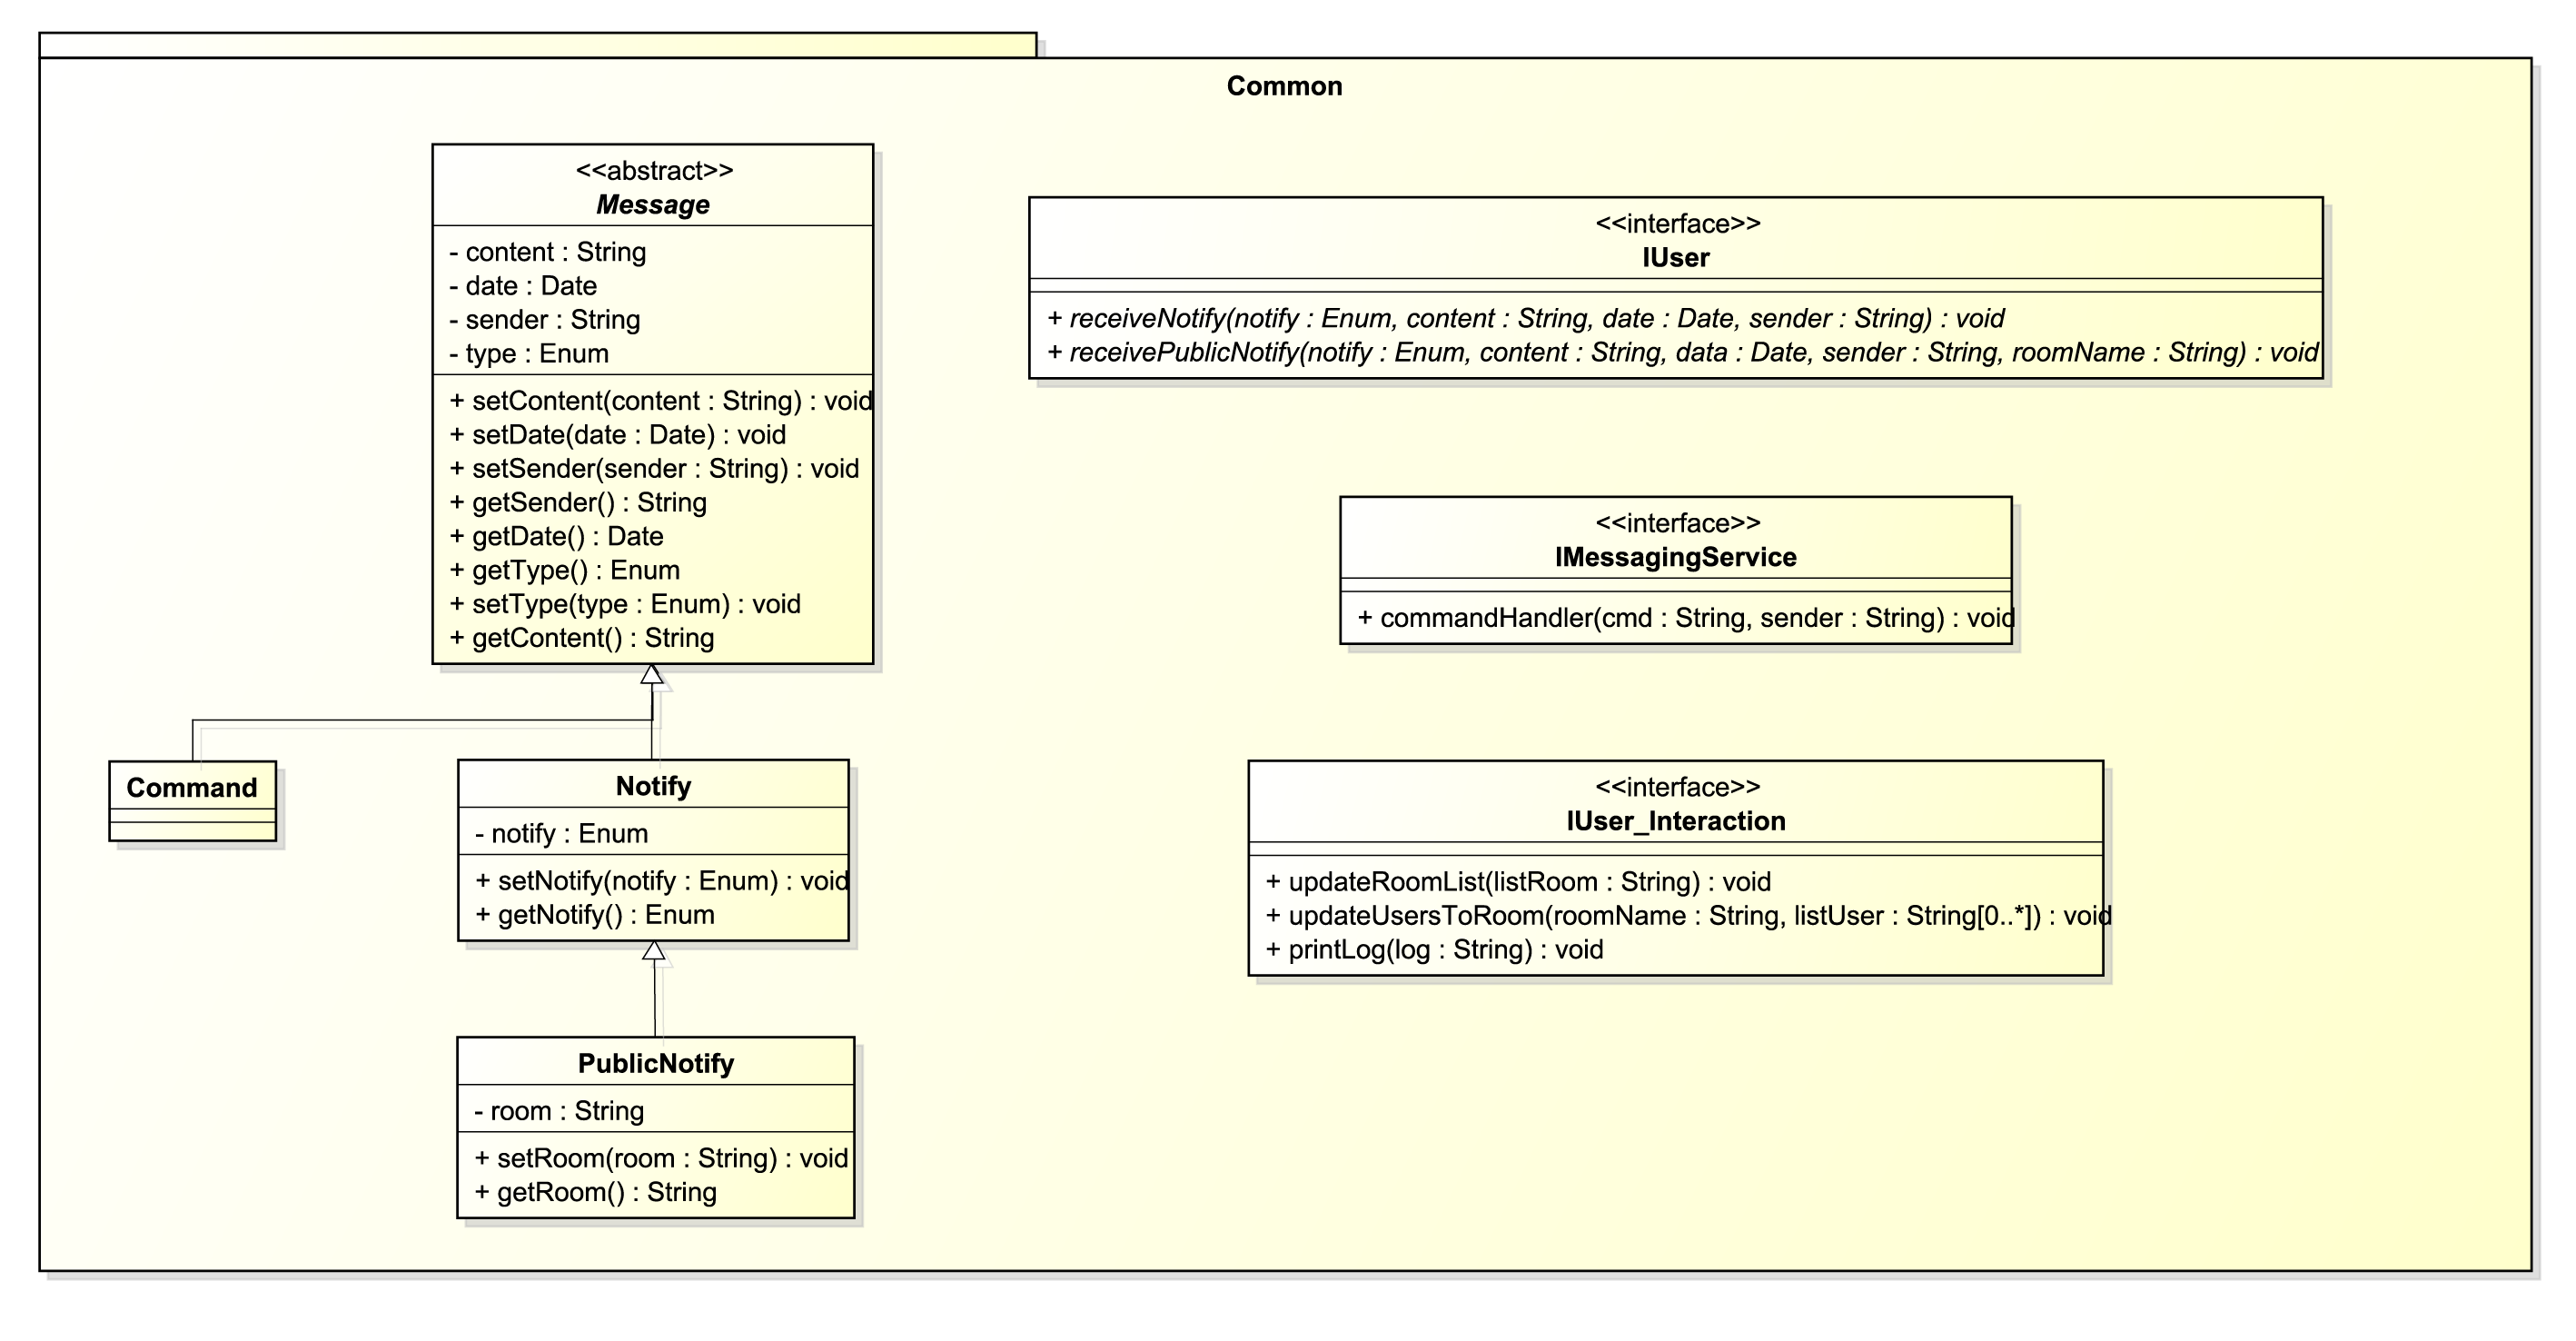
\includegraphics[scale=0.165]{image_astah/Iteration_1_DesignModel_Refactored/ClassDiagramCommon.png}{\centering}
     \caption{DCD - Diagramma delle Classi: Package Common }
     \label{fig_UC1_UC2_DCDR_1} 
   \end{figure}
\end{frame}

\begin{frame} {Refactoring Iterazione 1: Class Diagram Snuc UC1 e UC2}
   \begin{figure}
     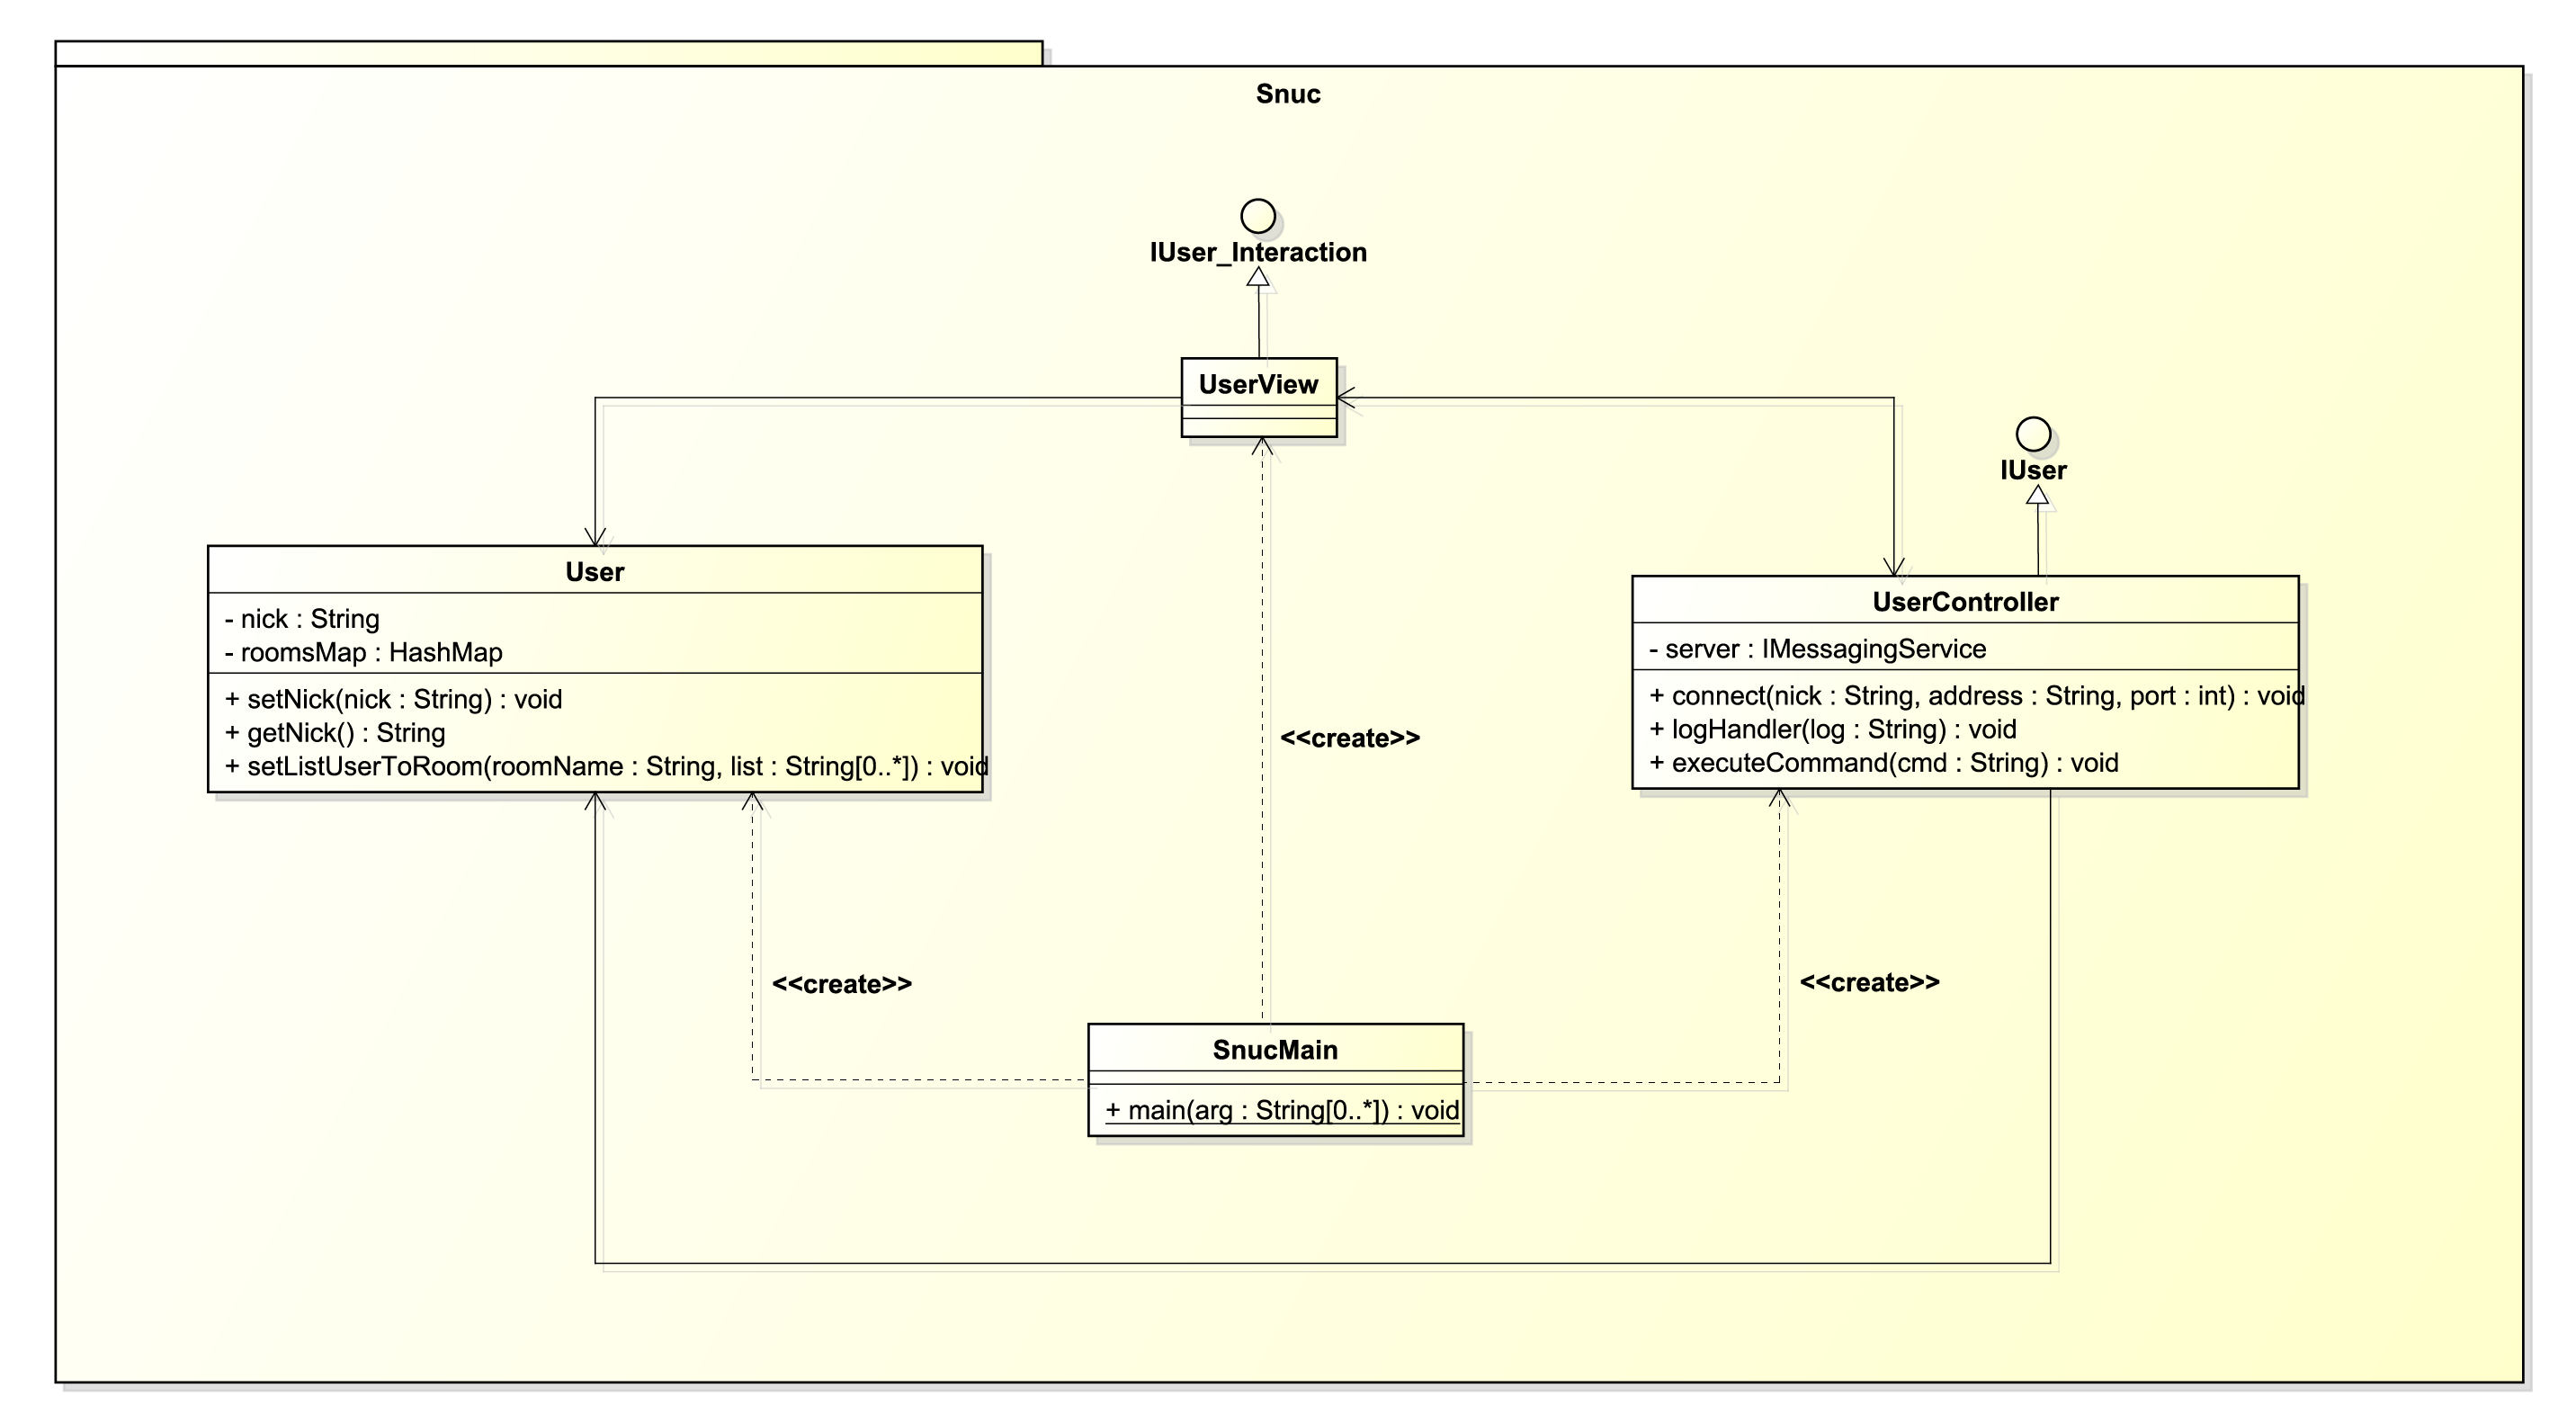
\includegraphics[scale=0.155]{image_astah/Iteration_1_DesignModel_Refactored/ClassDiagramSnuc.png}{\centering}
     \caption{DCD - Diagramma delle Classi: Package Snuc }
     \label{fig_UC1_UC2_DCDR_2} 
   \end{figure}
\end{frame}

\begin{frame} {Refactoring Iterazione 1: Class Diagram Connector UC1 e UC2}
   \begin{figure}
     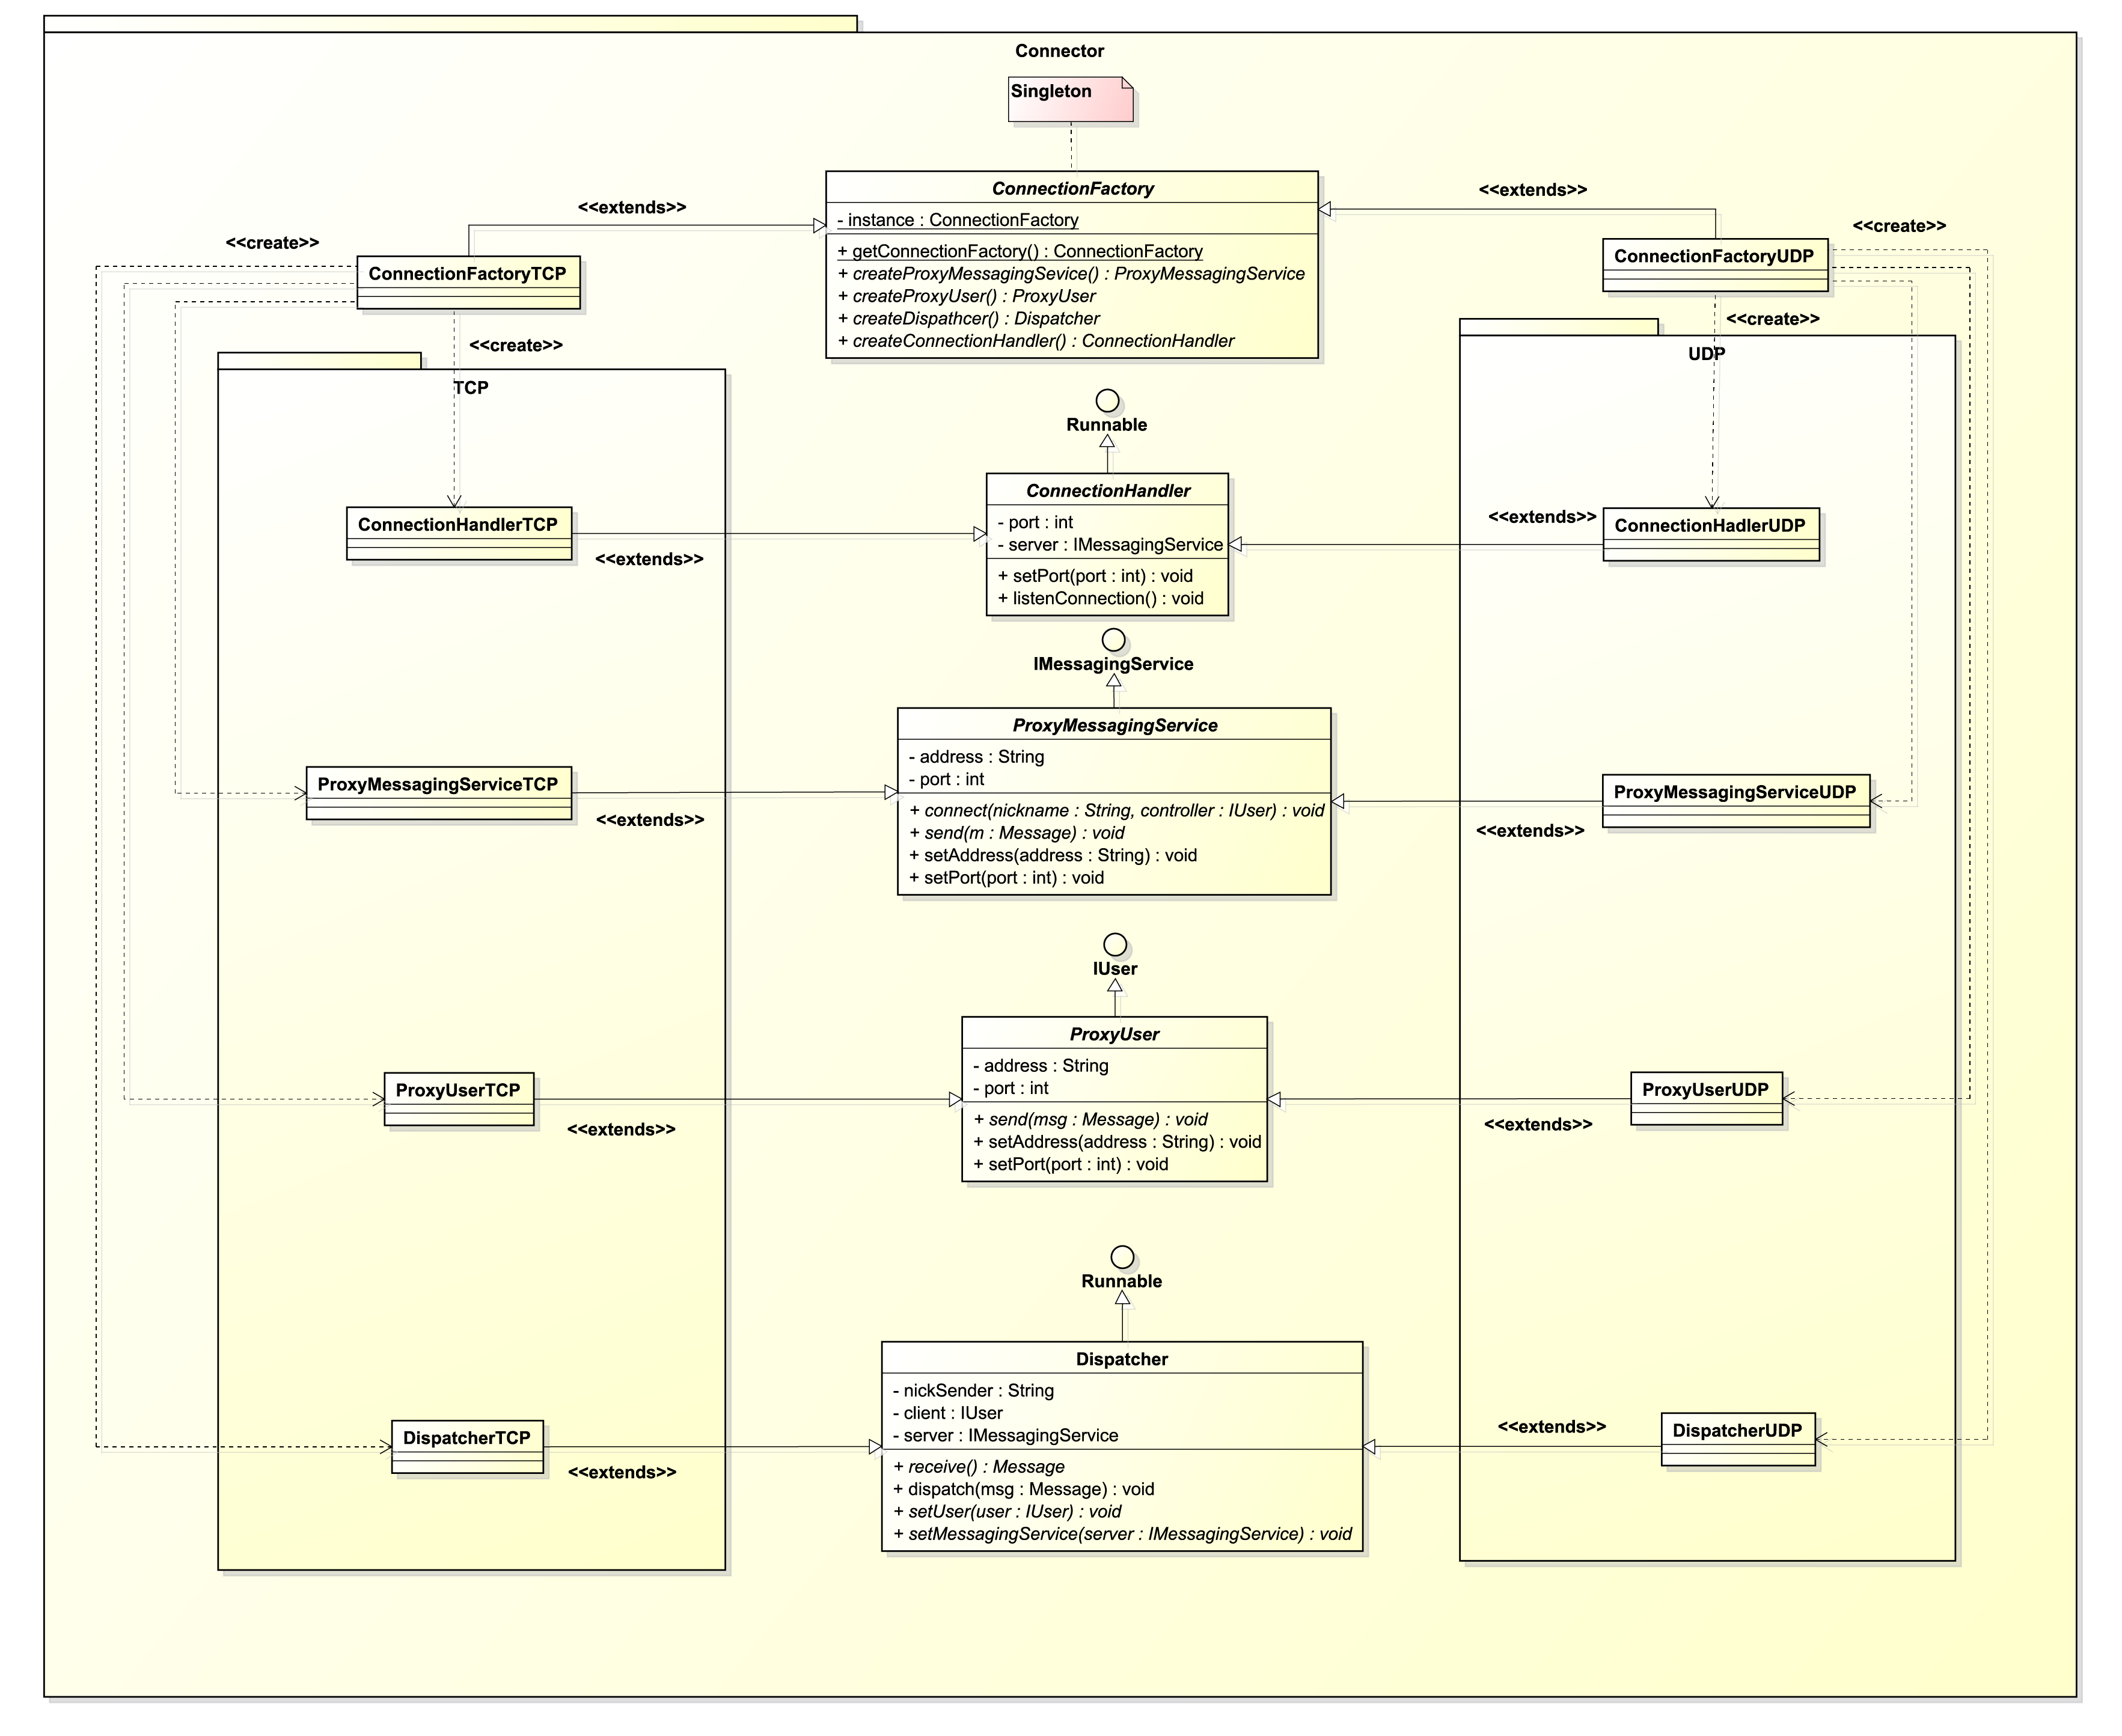
\includegraphics[scale=0.084]{image_astah/Iteration_1_DesignModel_Refactored/ClassDiagramConnector.png}{\centering}
     \caption{DCD - Diagramma delle Classi: Package Connector }
     \label{fig_UC1_UC2_DCDR_3} 
   \end{figure}
\end{frame}

\begin{frame} {Refactoring Iterazione 1: Class Diagram Snuc Server UC1 e UC2}
   \begin{figure}
     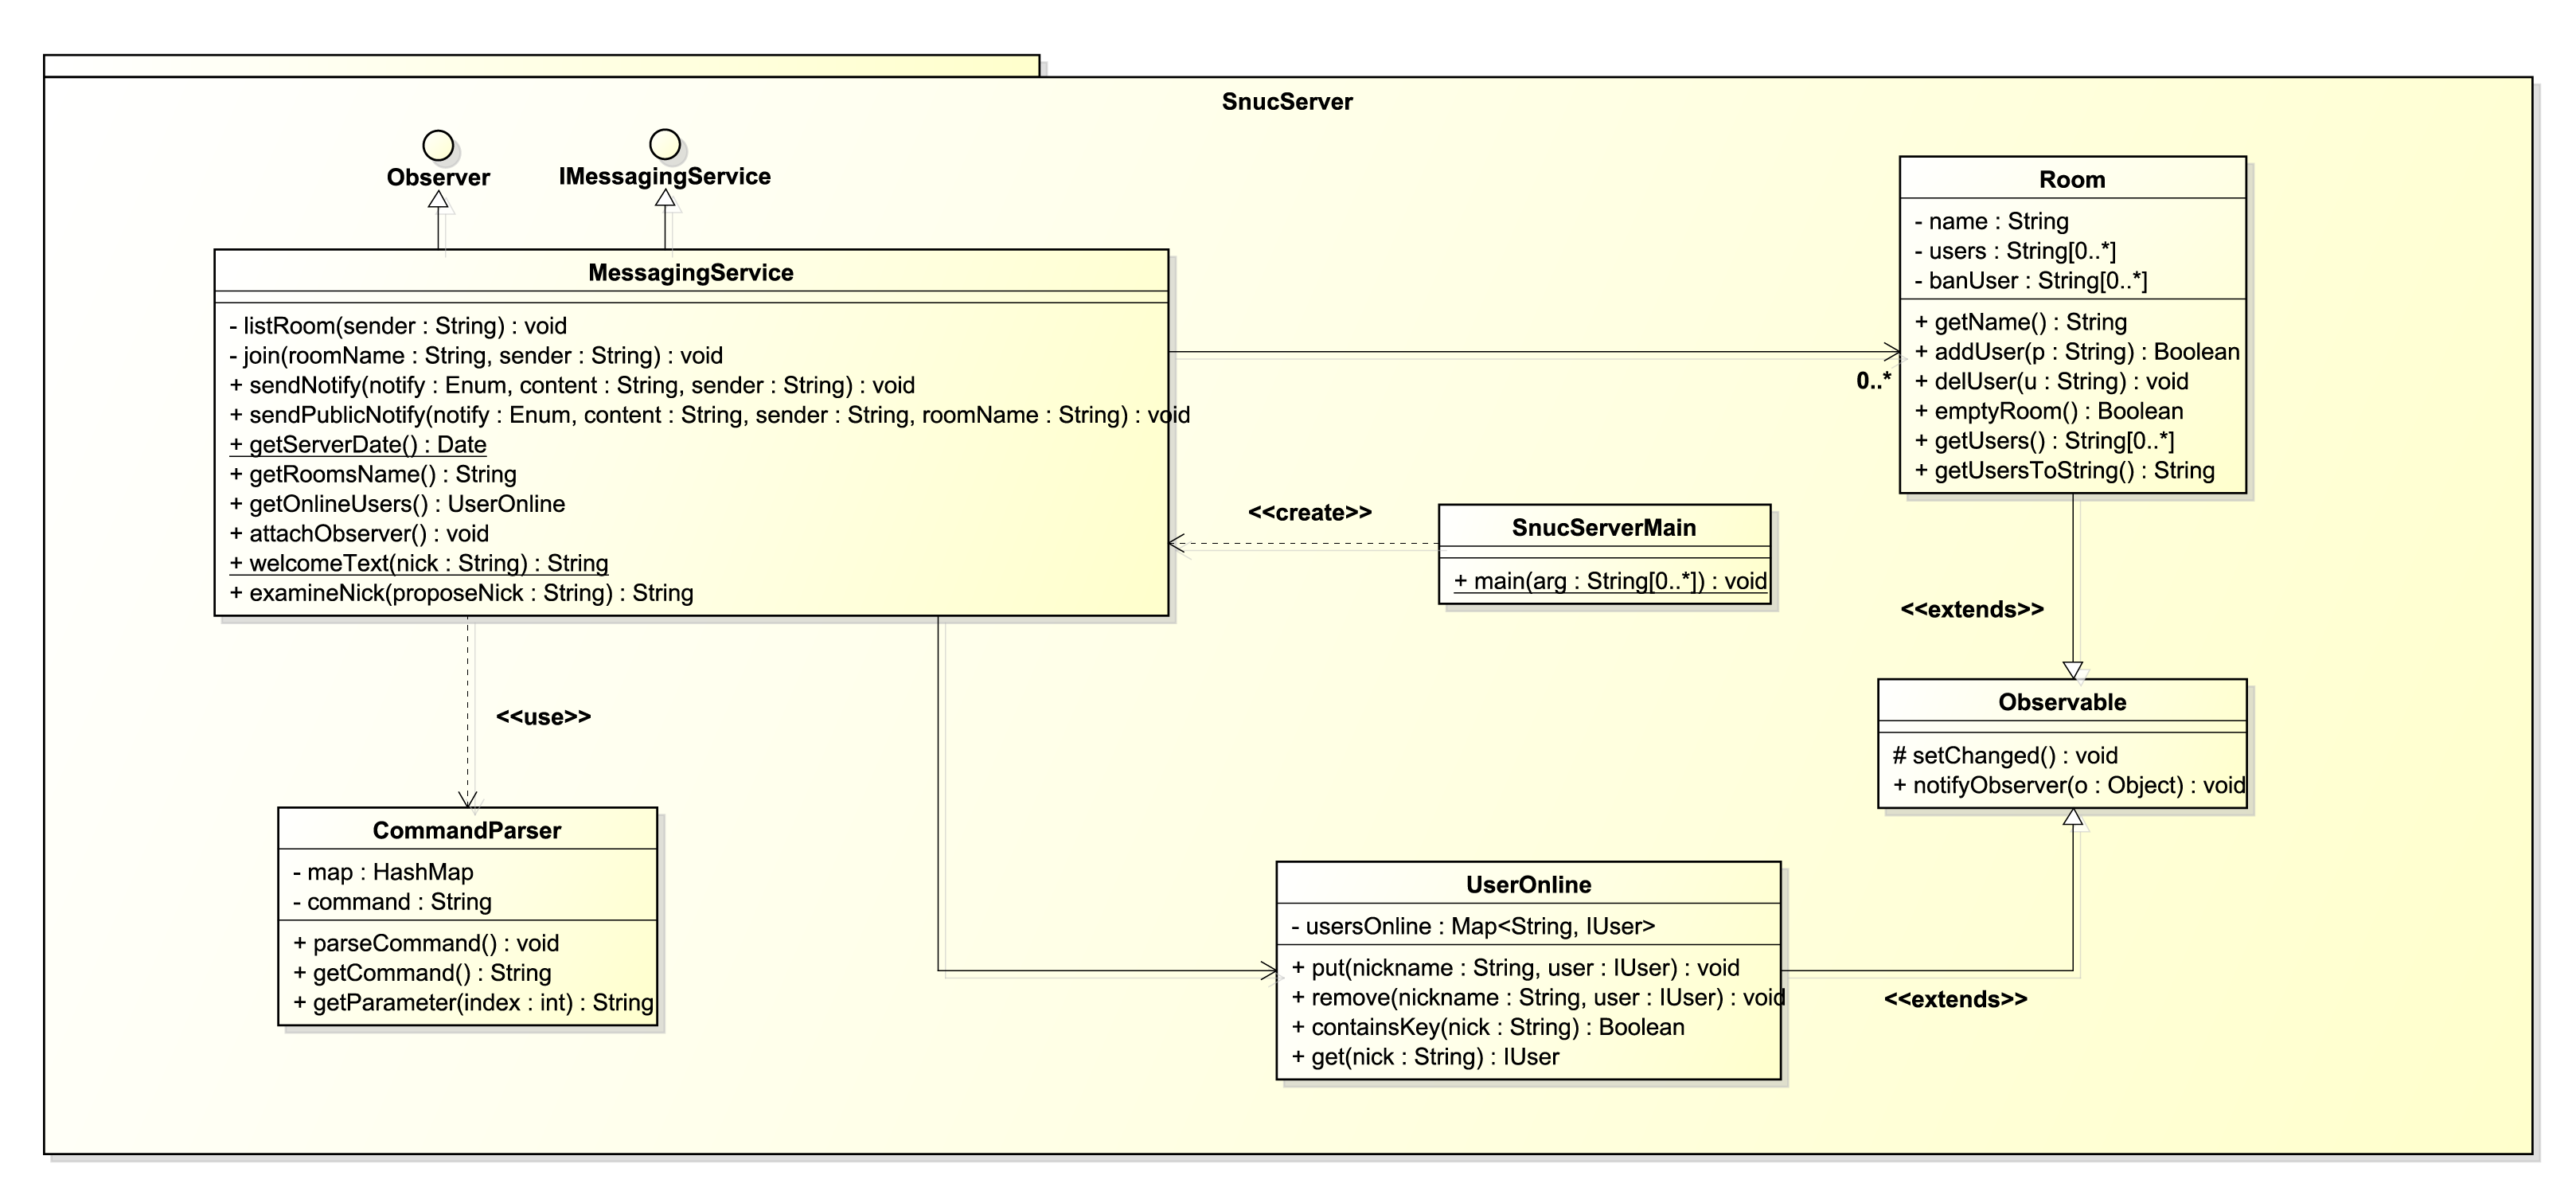
\includegraphics[scale=0.144]{image_astah/Iteration_1_DesignModel_Refactored/ClassDiagramSnucServer.png}{\centering}
     \caption{DCD - Diagramma delle Classi: Package Snuc Server }
     \label{fig_UC1_UC2_DCDR_4} 
   \end{figure}
\end{frame}

\subsection{Refactoring Iterazione 1: SSD UC1 e UC2}
\begin{frame} {Refactoring Iterazione 1: UC1\_RequestConnection}
   \begin{figure}
     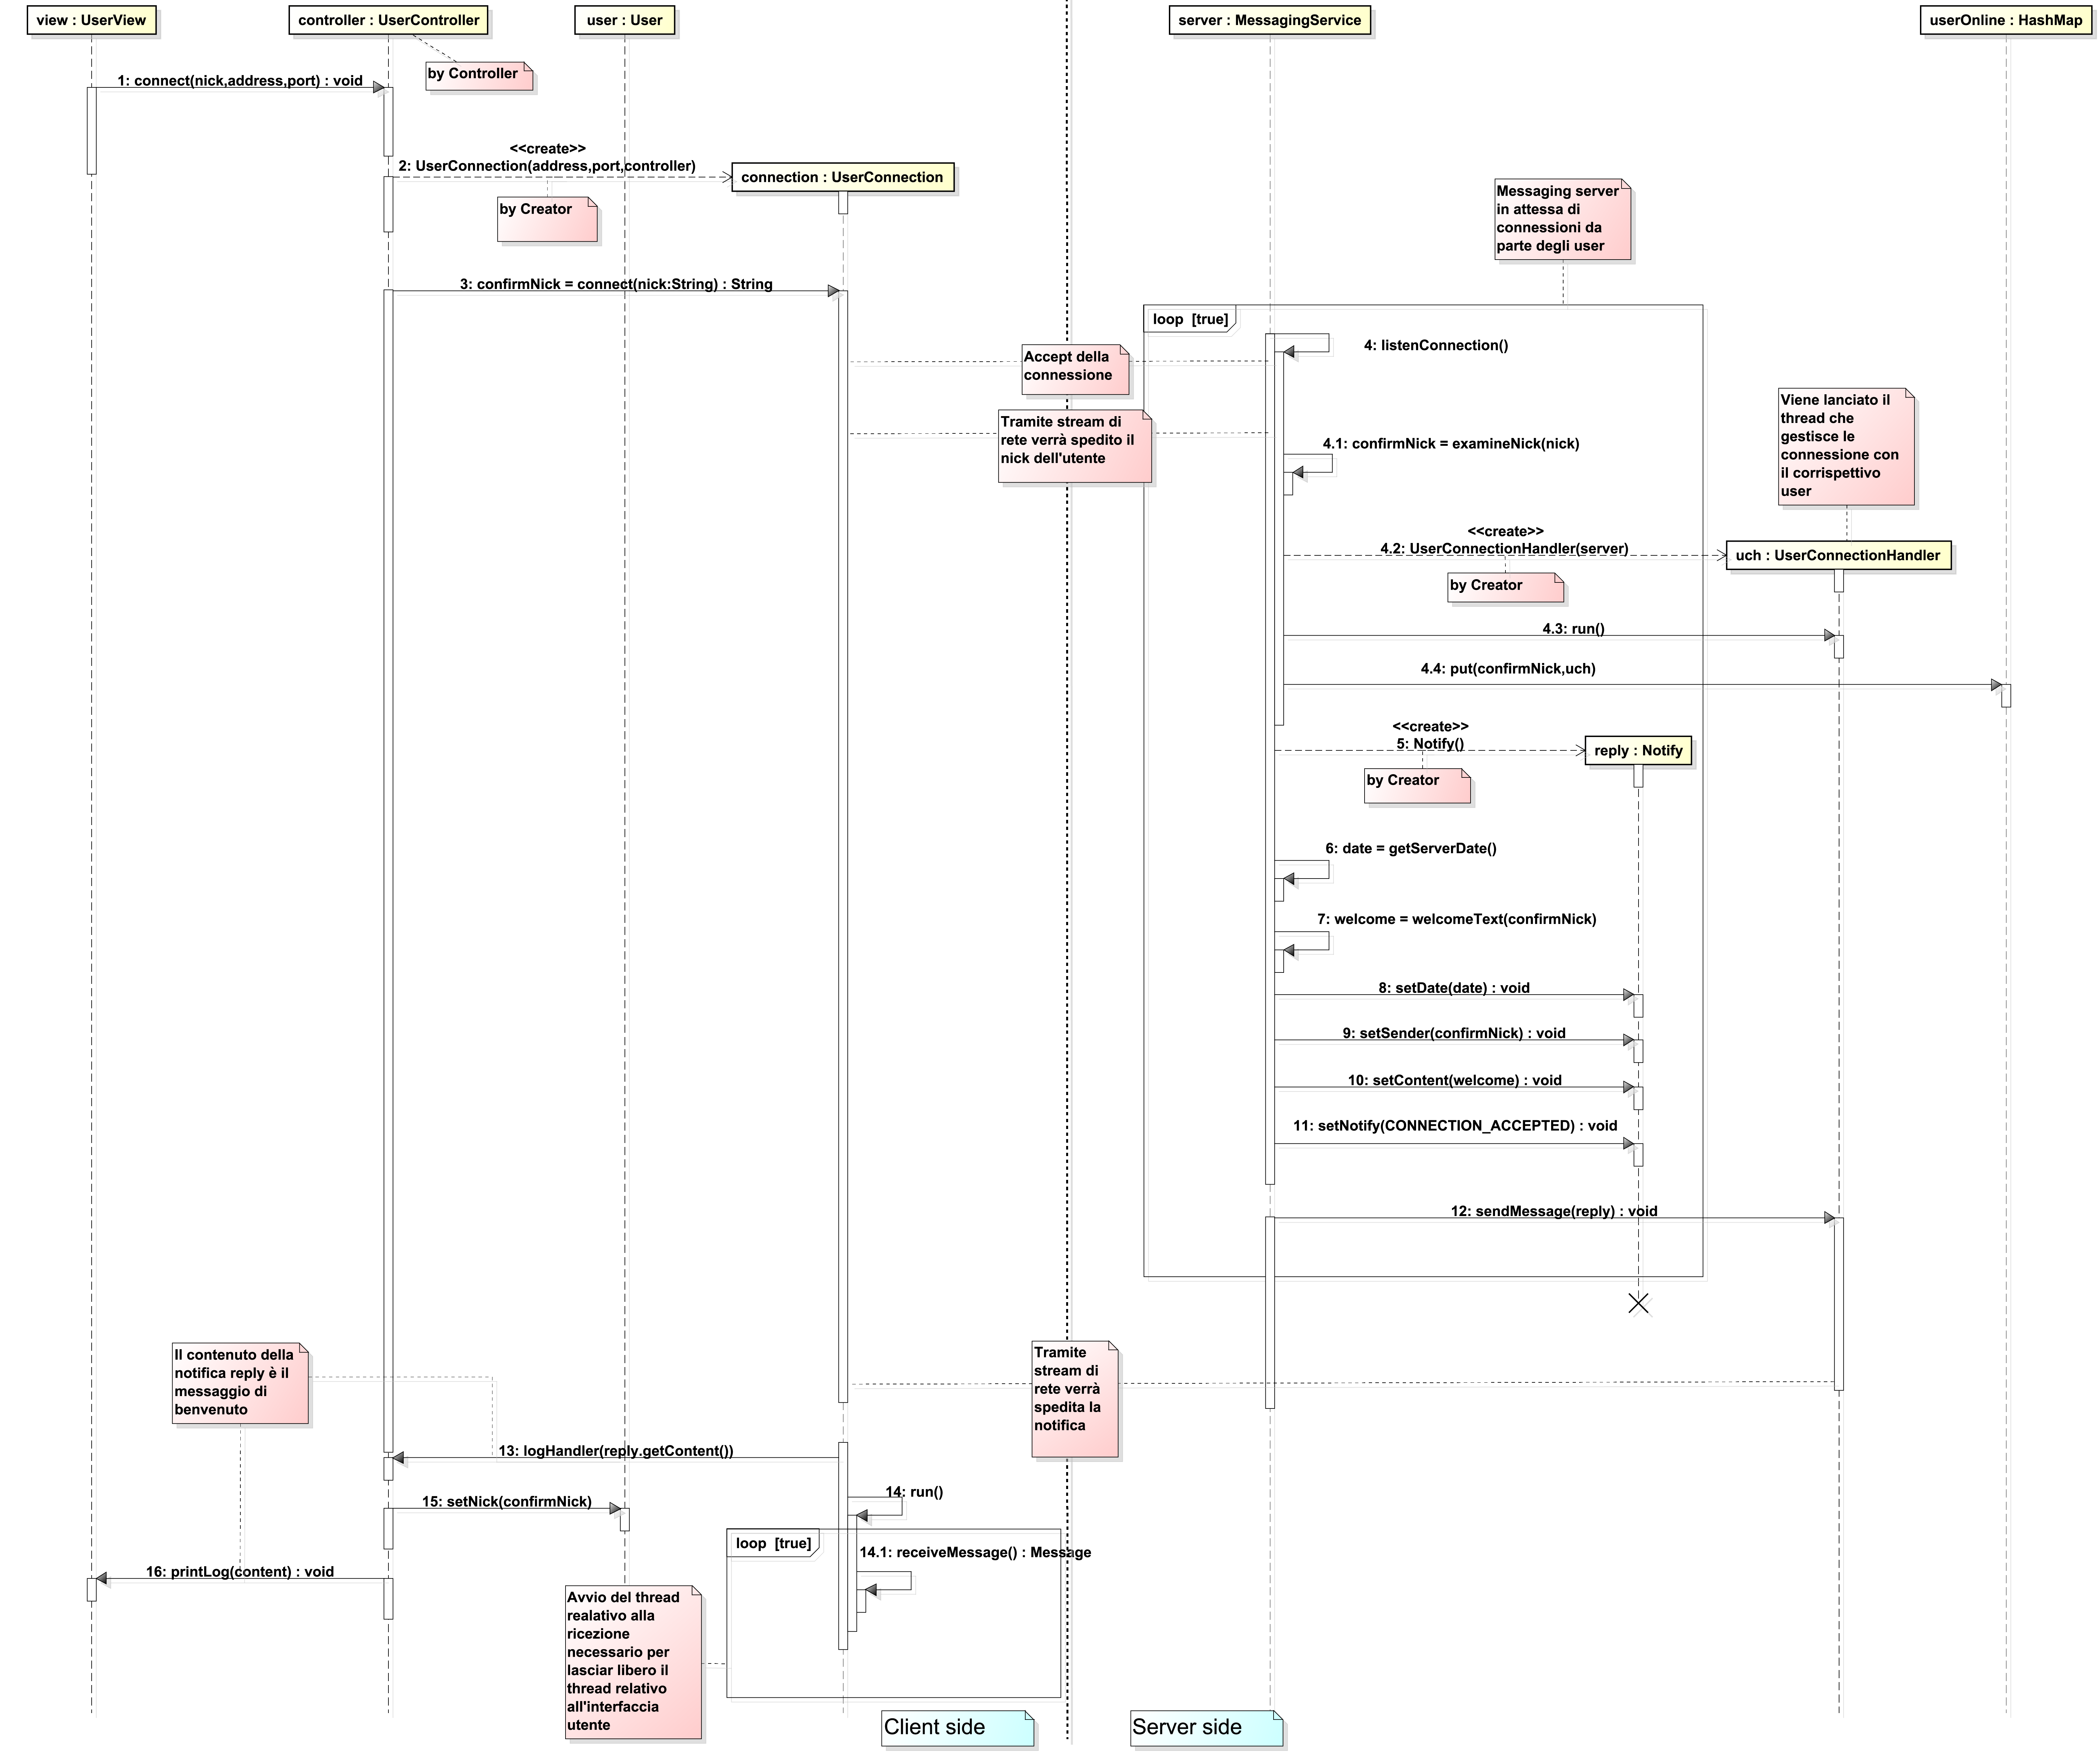
\includegraphics[scale=0.0475]{image_astah/Iteration_1_DesignModel_Refactored/UC1_RequestConnection_SSD_3_4_connect.png}{\centering}
     \caption{SSD - OP1-4: connect(nick), notify(response) del modello dominio (figura \ref{fig_UC1_RC_SSD}) }
     \label{fig_UC1_SSDR_RC_1_4} 
   \end{figure}
\end{frame}

\begin{frame} {Refactoring Iterazione 1: UC2\_AccessRoom - OP1}
   \begin{figure}
     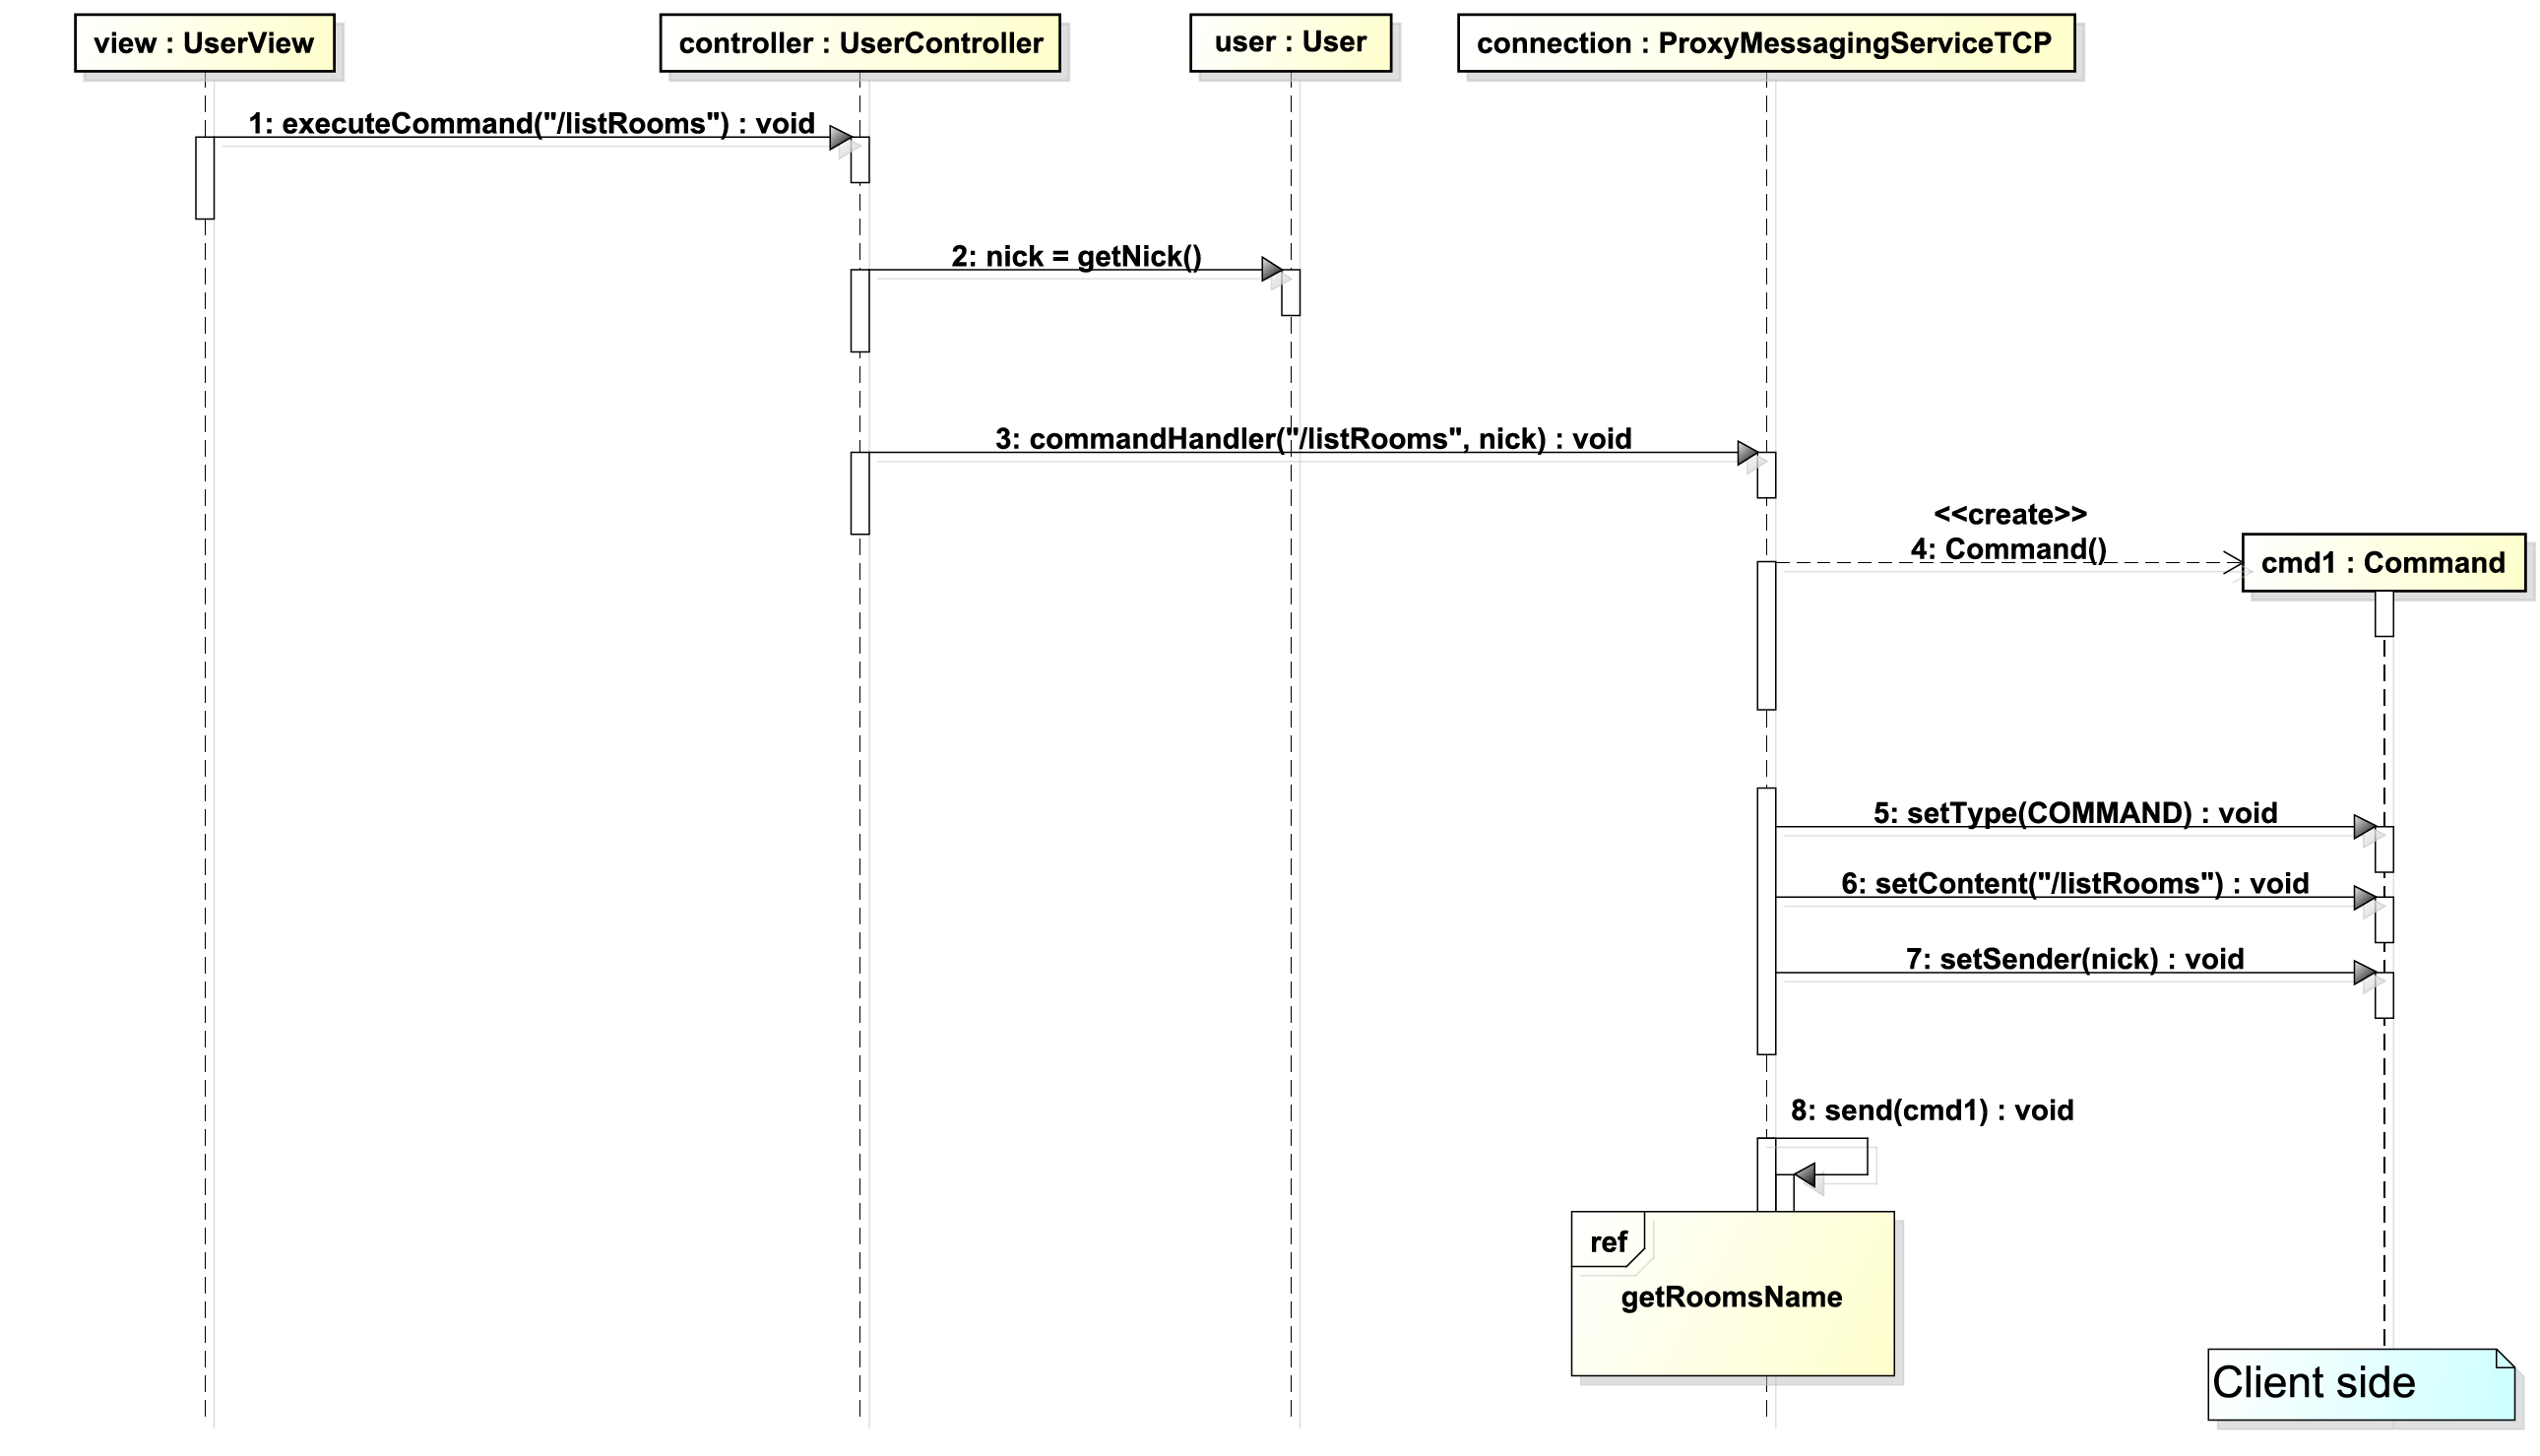
\includegraphics[scale=0.16]{image_astah/Iteration_1_DesignModel_Refactored/UC2_AccessRoom_SSD_1_sendCommand.png}{\centering}
     \caption{SSD - OP1: sendCommand(cmd1) del modello di dominio (figura \ref{fig_UC2_AR_SSD}) }
     \label{fig_UC2_SSDR_AC_1} 
   \end{figure}
\end{frame}

\begin{frame} {Refactoring Iterazione 1: UC2\_AccessRoom - OP2}
   \begin{figure}
     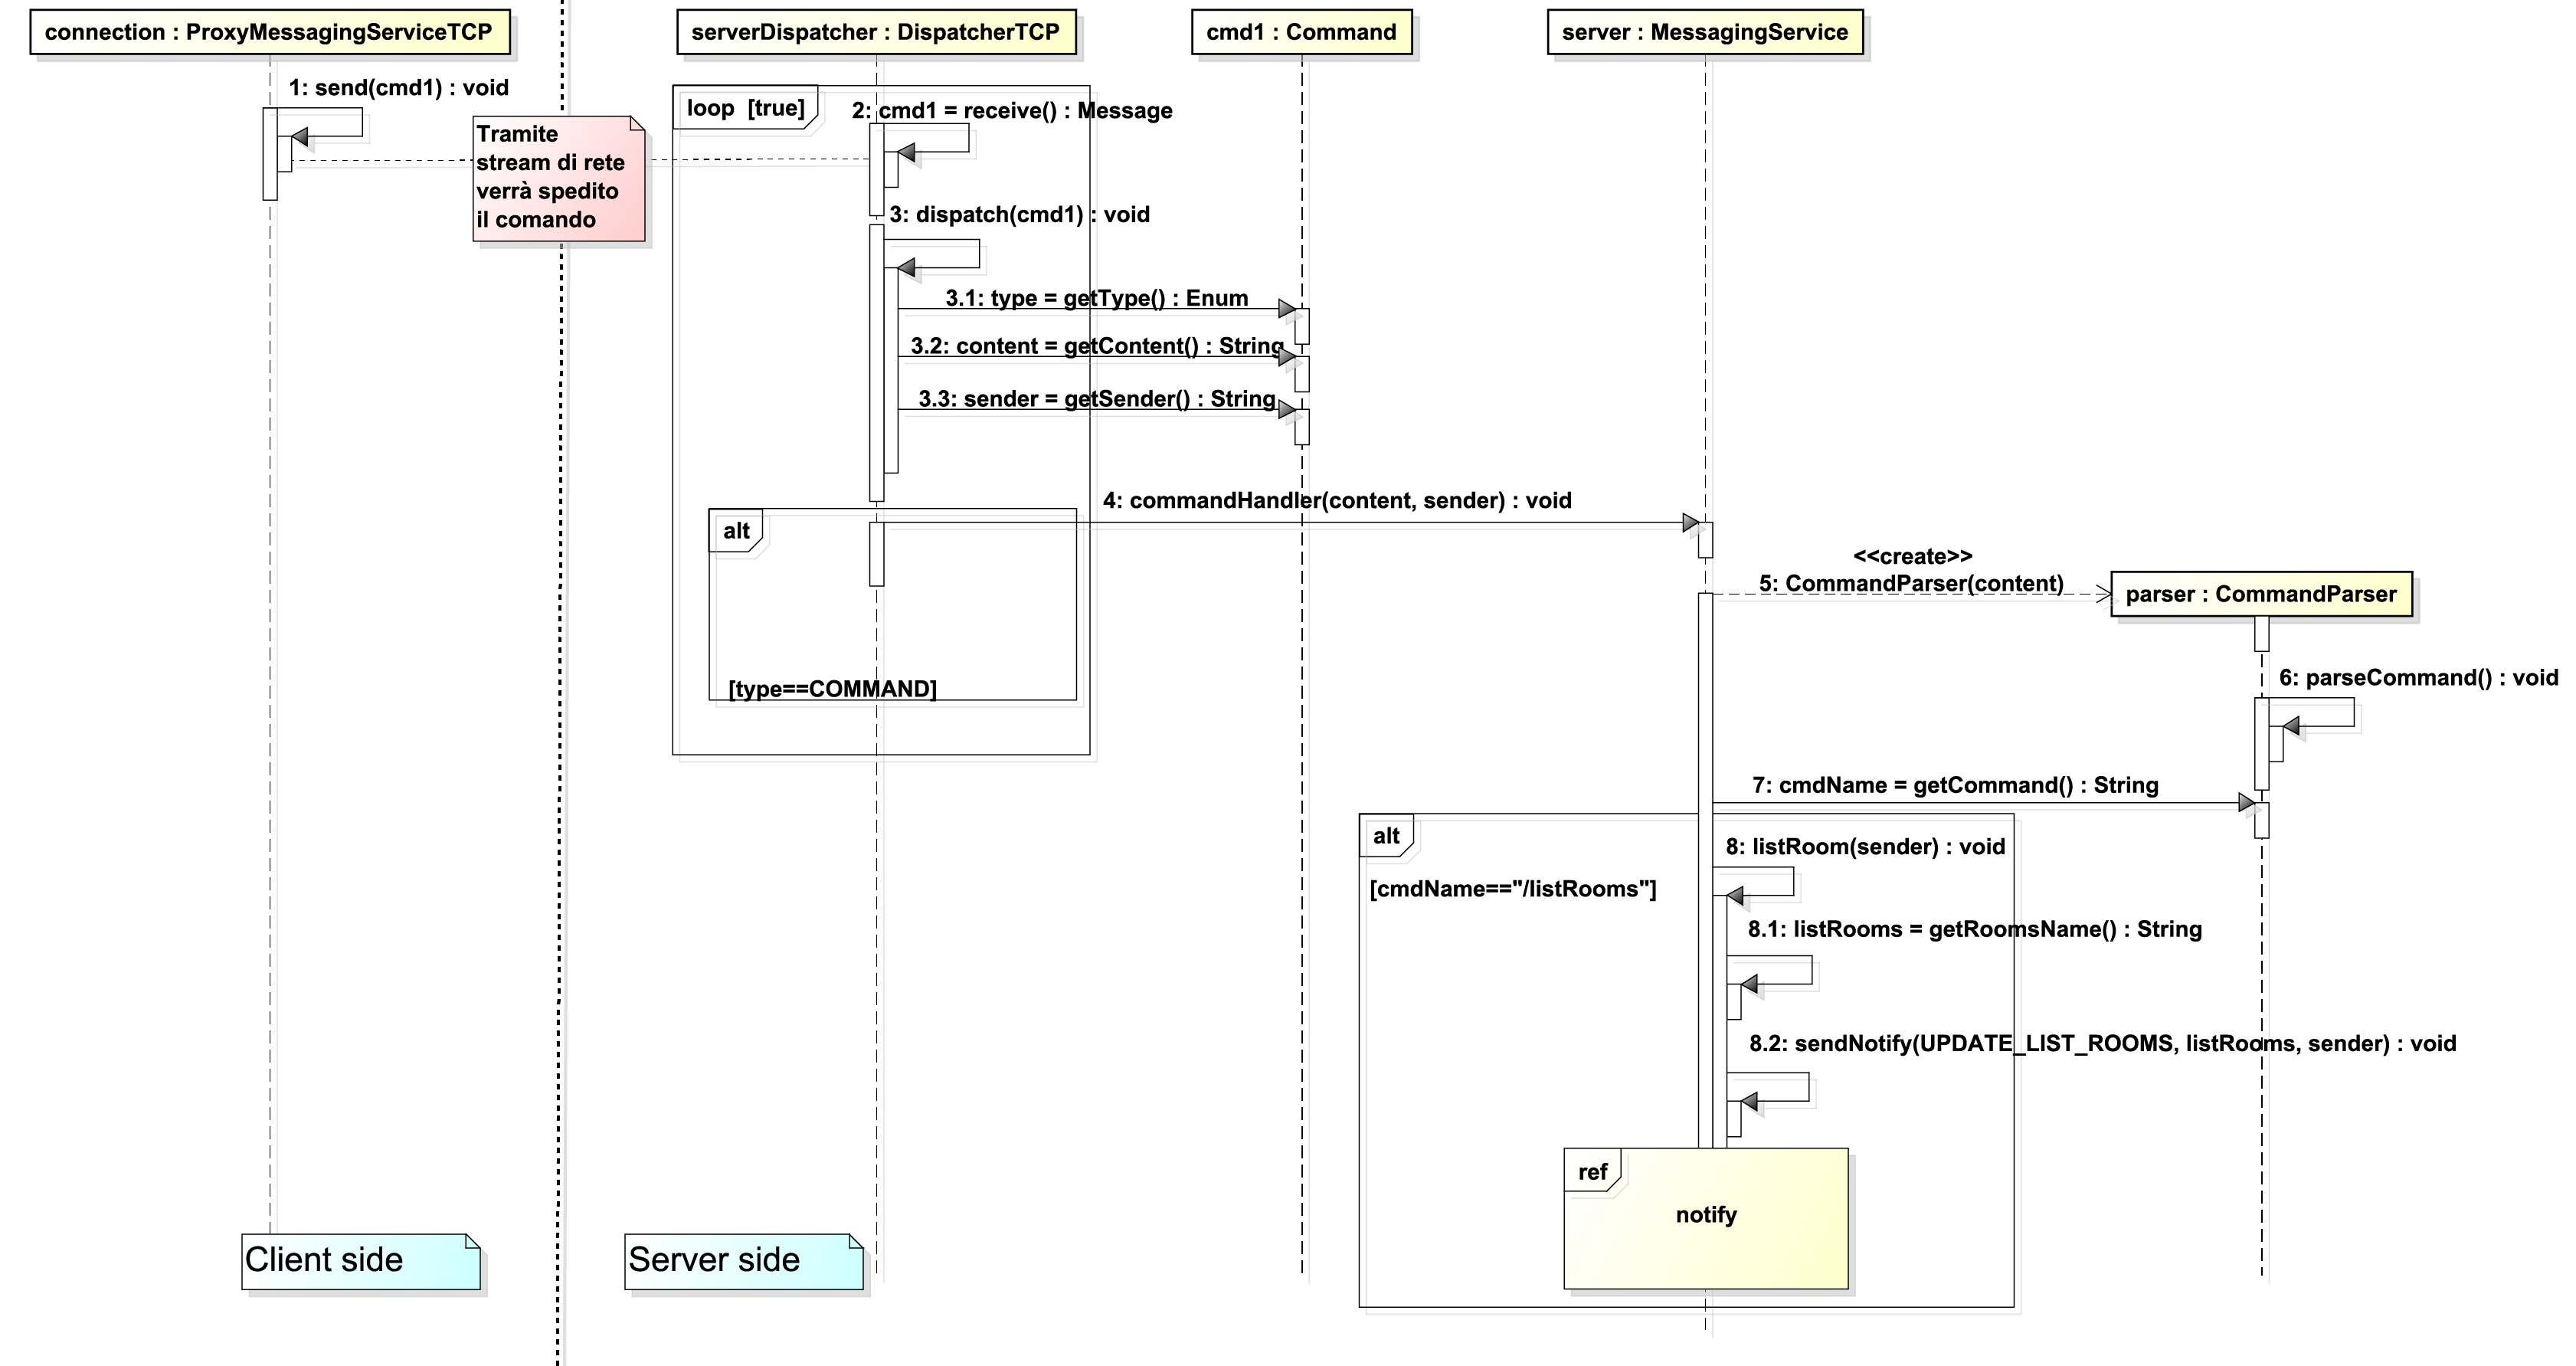
\includegraphics[scale=0.135]{image_astah/Iteration_1_DesignModel_Refactored/UC2_AccessRoom_SSD_2_getRoomsName.png}{\centering}
     \caption{SSD - OP2: getRoomsName() del modello di dominio (figura \ref{fig_UC2_AR_SSD}) }
     \label{fig_UC2_SSDR_AC_2} 
   \end{figure}
\end{frame}

\begin{frame} {Refactoring Iterazione 1: UC2\_AccessRoom - OP3}
   \begin{figure}
     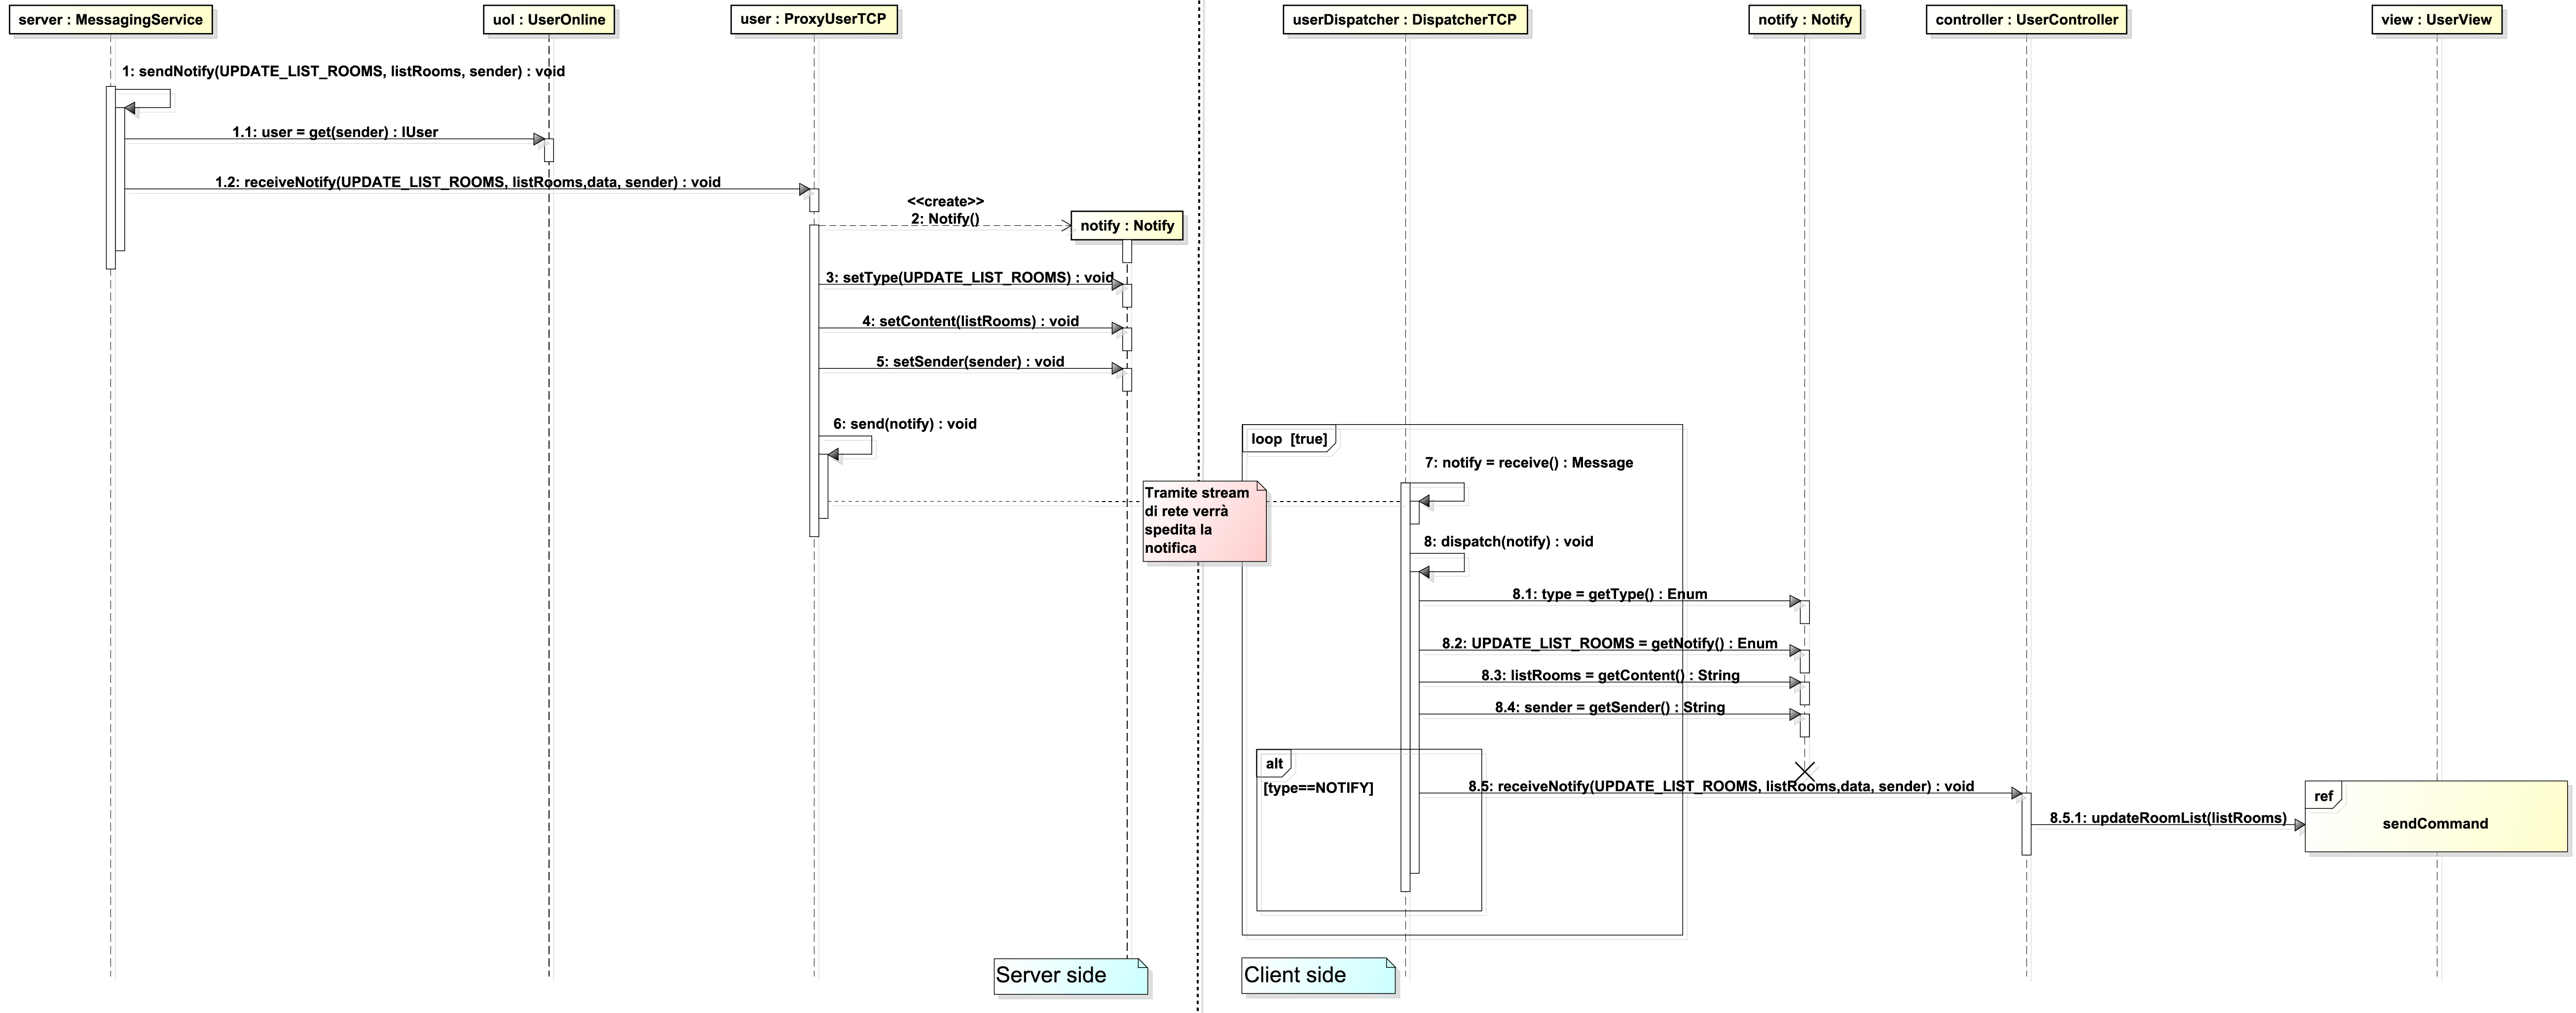
\includegraphics[scale=0.085]{image_astah/Iteration_1_DesignModel_Refactored/UC2_AccessRoom_SSD_3_notify.png}{\centering}
     \caption{SSD - OP3: notify(list) del modello di dominio (figura \ref{fig_UC2_AR_SSD})}
     \label{fig_UC2_SSDR_AC_3} 
   \end{figure}
\end{frame}

\begin{frame} {Refactoring Iterazione 1: UC2\_AccessRoom - OP4}
   \begin{figure}
     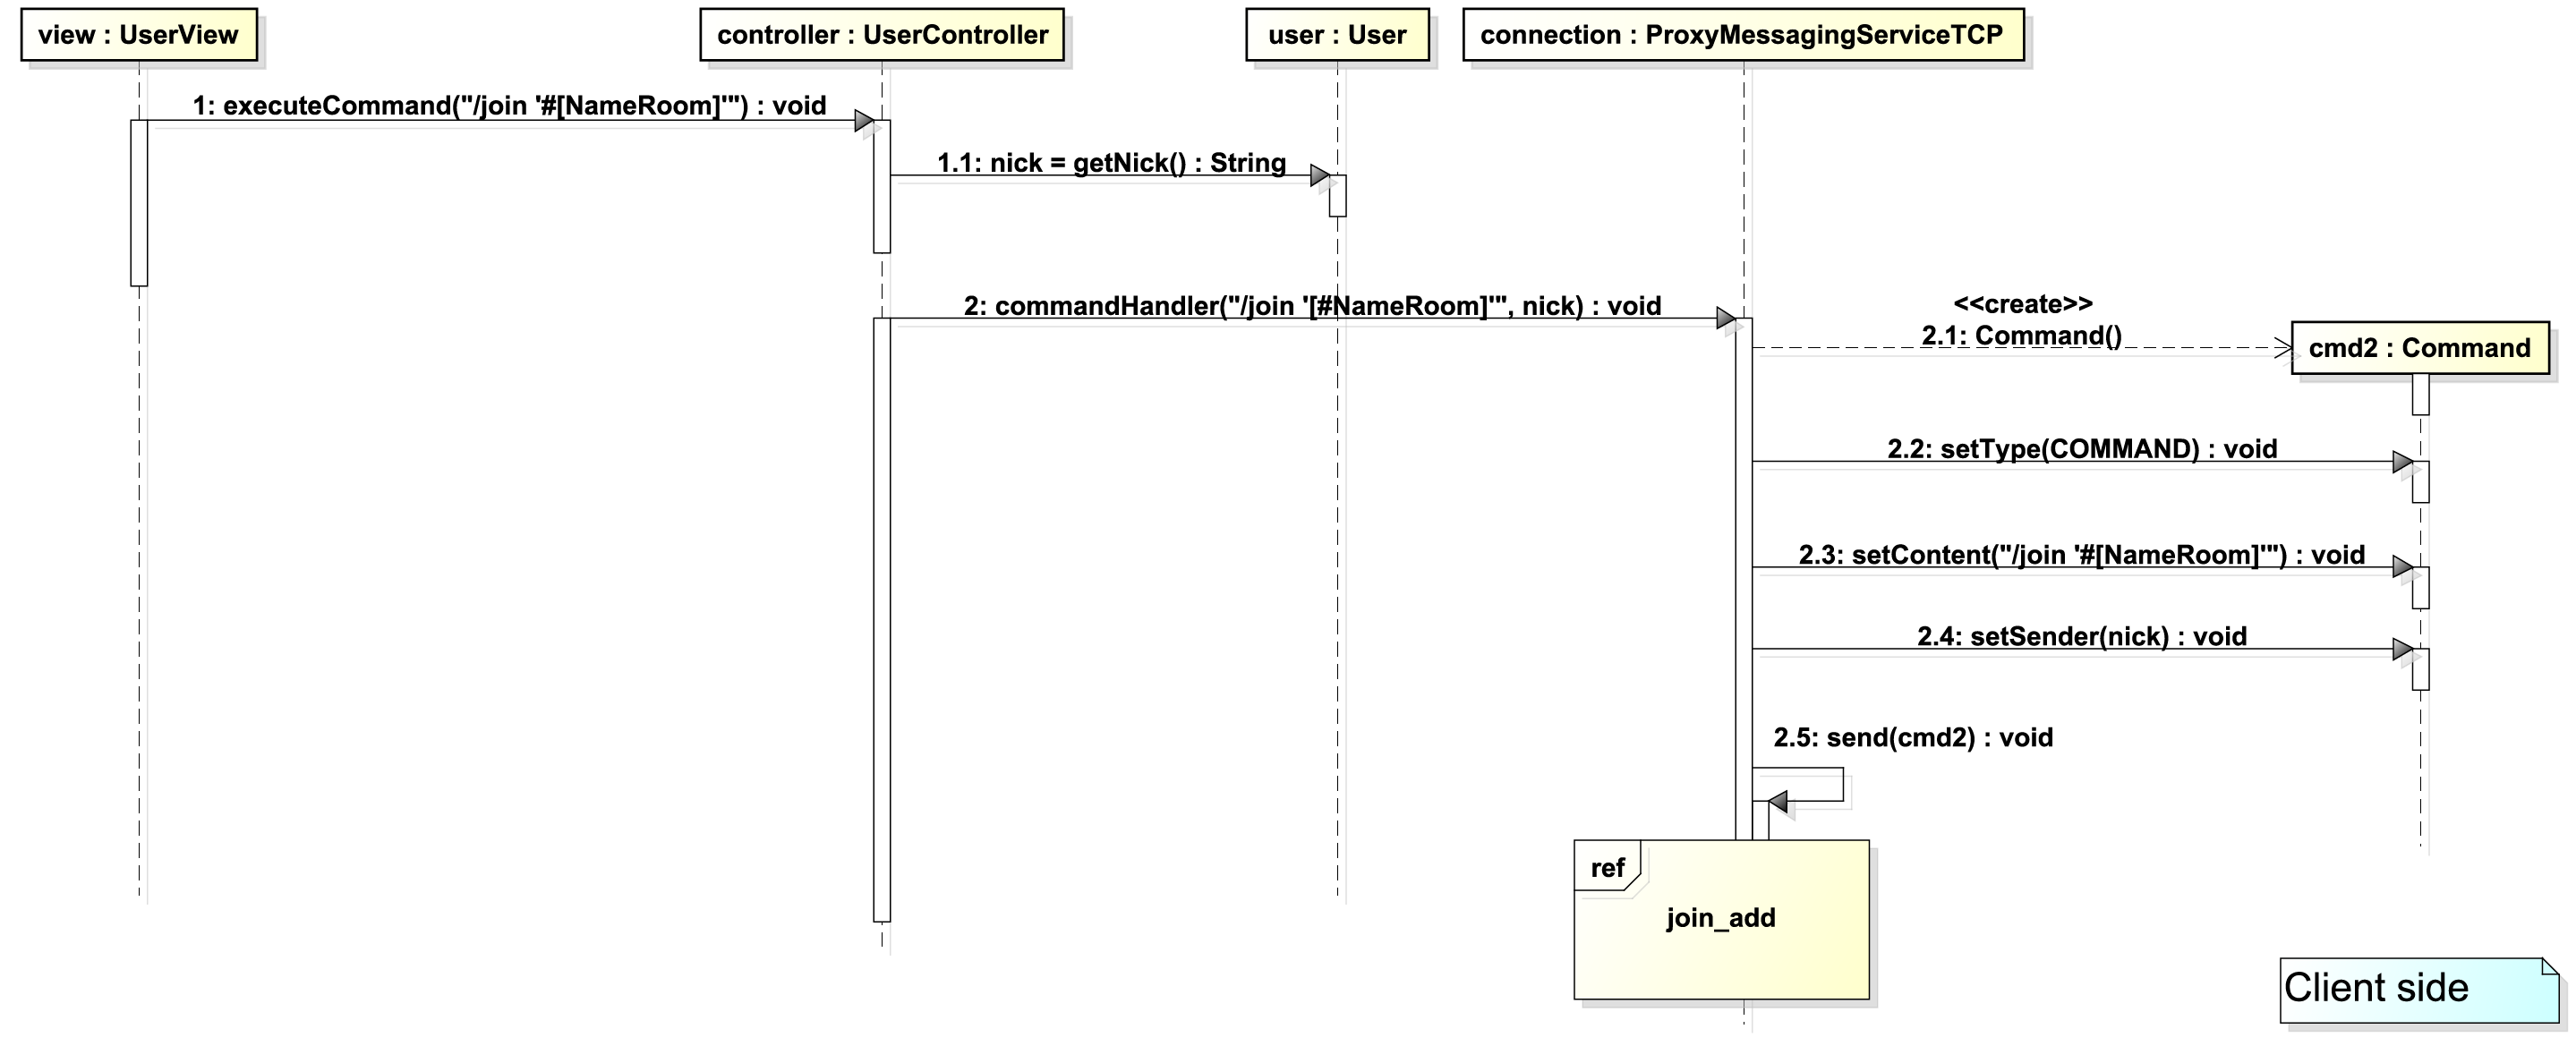
\includegraphics[scale=0.158]{image_astah/Iteration_1_DesignModel_Refactored/UC2_AccessRoom_SSD_4_sendCommand.png}{\centering}
     \caption{SSD - OP4: sendCommand(cmd2) del modello di dominio (figura \ref{fig_UC2_AR_SSD}) }
     \label{fig_UC2_SSDR_AC_4} 
   \end{figure}
\end{frame}

\begin{frame} {Refactoring Iterazione 1: UC2\_AccessRoom - OP5}
   \begin{figure}
     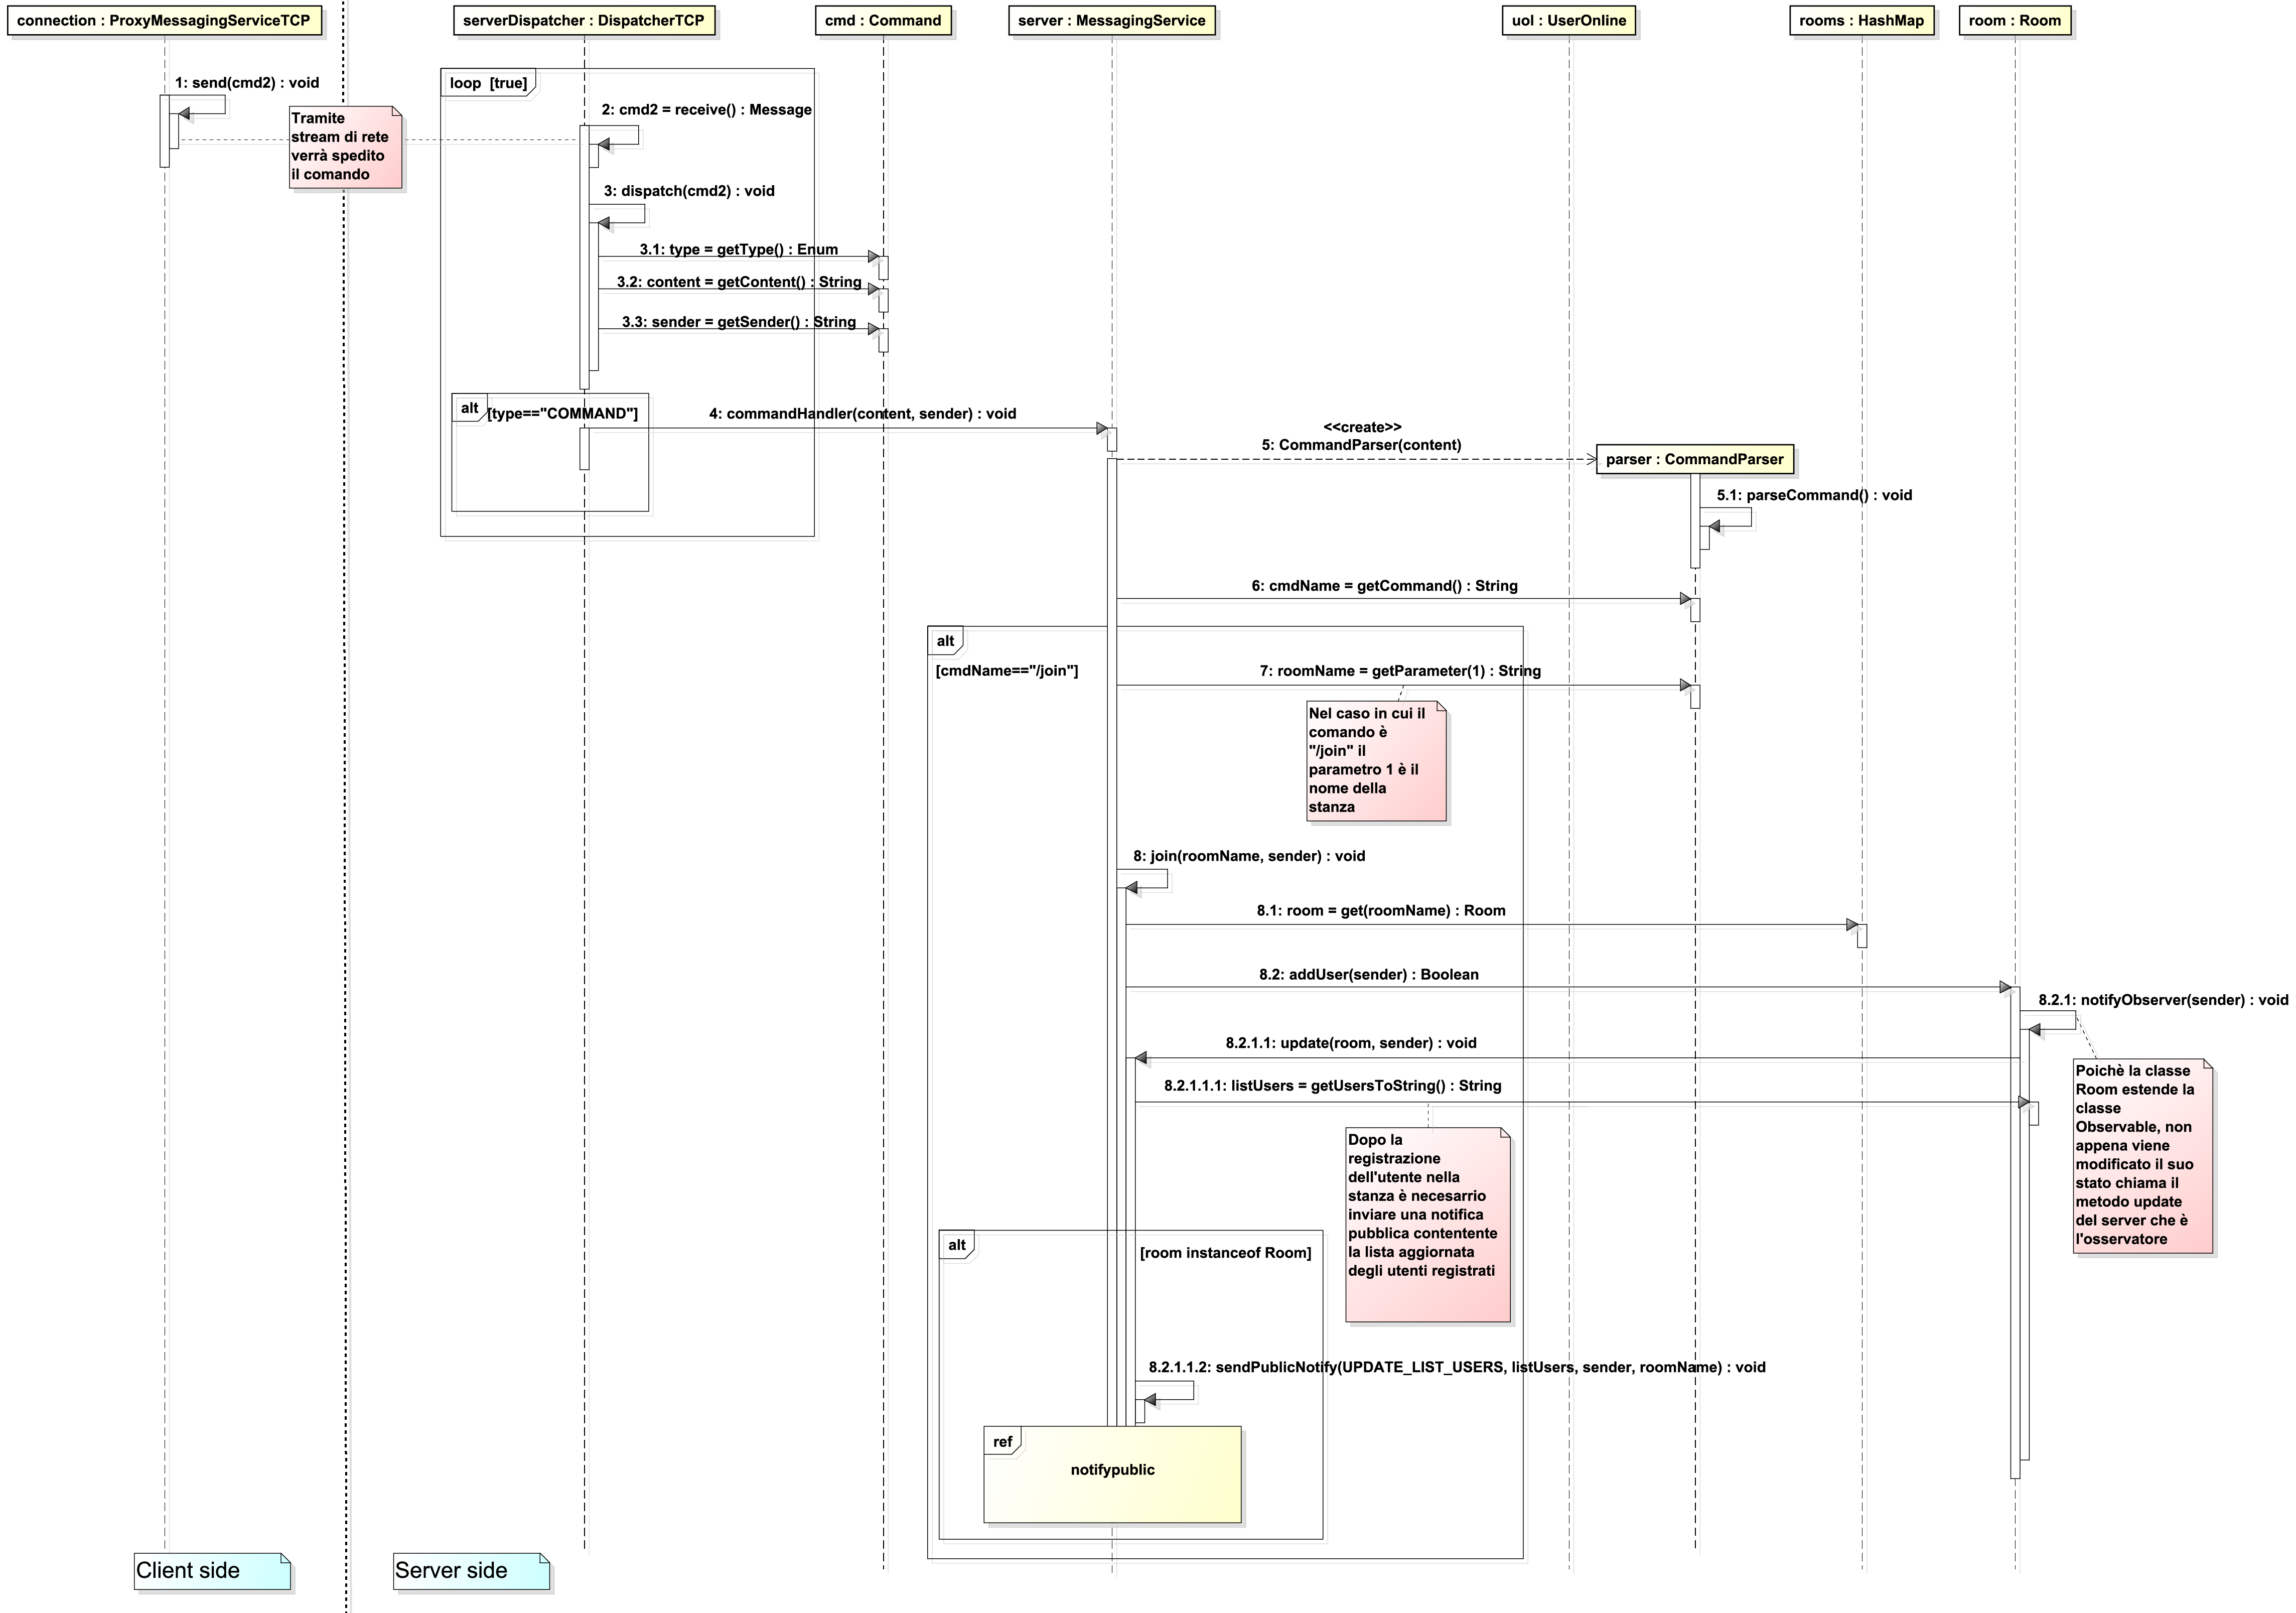
\includegraphics[scale=0.075]{image_astah/Iteration_1_DesignModel_Refactored/UC2_AccessRoom_SSD_5_join_add.png}{\centering}
     \caption{SSD - OP5: joinRoom(sender,room), addUserToRoom() del modello di dominio (figura \ref{fig_UC2_AR_SSD}) }
     \label{fig_UC2_SSDR_AC_5} 
   \end{figure}
\end{frame}

\begin{frame} {Refactoring Iterazione 1: UC2\_AccessRoom - OP6}
   \begin{figure}
     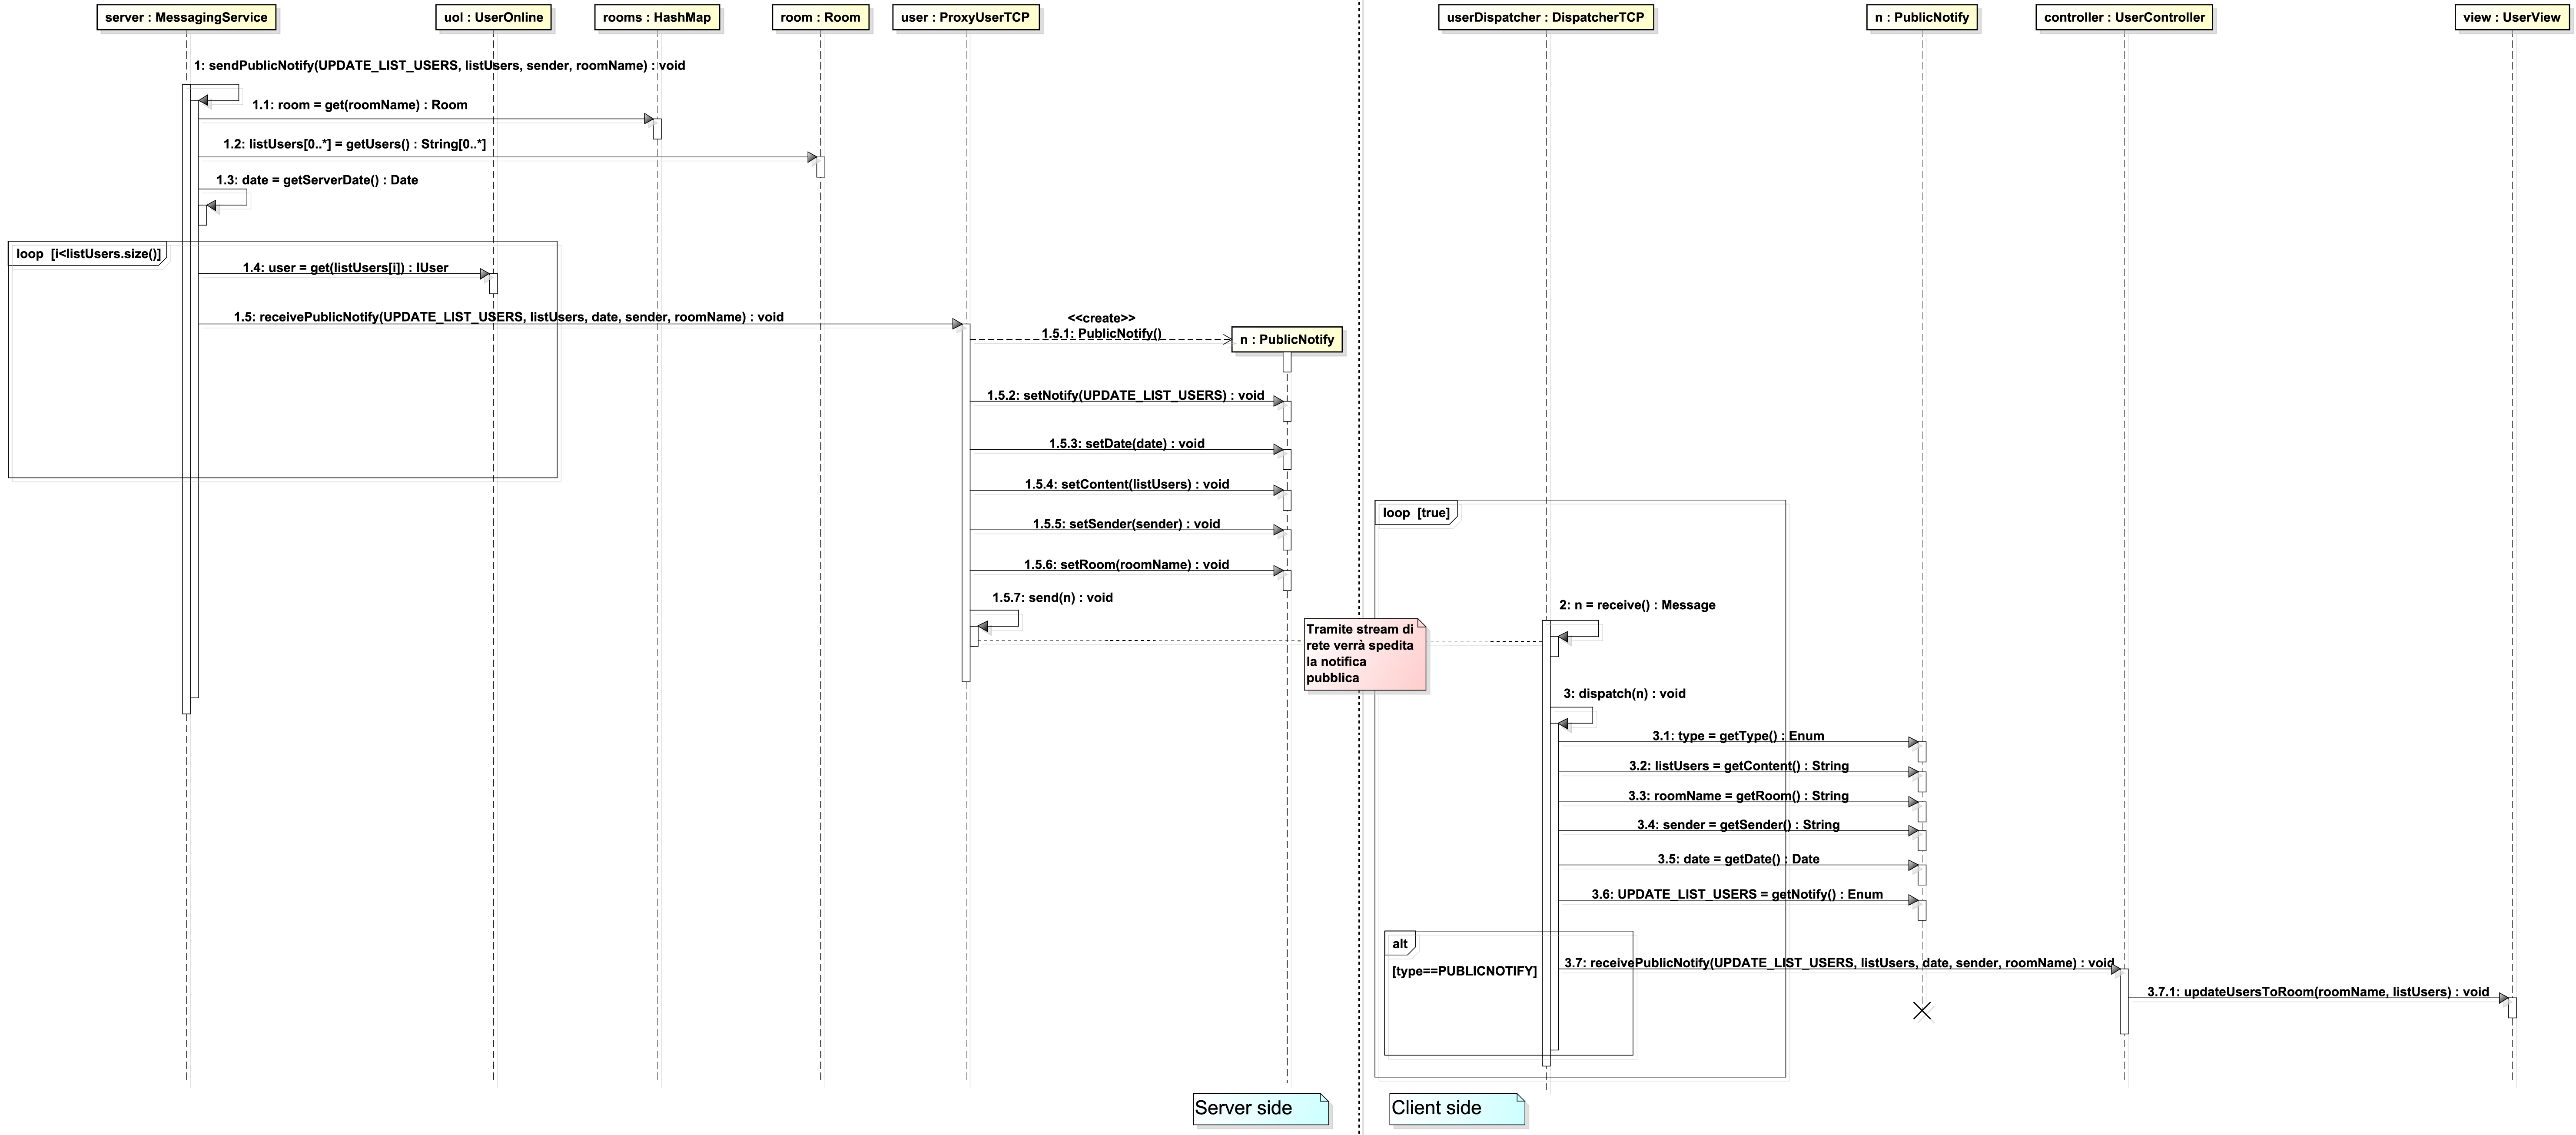
\includegraphics[scale=0.077]{image_astah/Iteration_1_DesignModel_Refactored/UC2_AccessRoom_SSD_6_notifypublic.png}{\centering}
     \caption{SSD - OP6: notifypublic(updateList) del modello di dominio (figura \ref{fig_UC2_AR_SSD}) }
     \label{fig_UC2_SSDR_AC_6} 
   \end{figure}
\end{frame}

\subsection{Refactoring Iterazione 1: Implementazione UC1 e UC2}
\begin{frame} {Refactoring Iterazione 1: Implementazione UC1 e UC2}
 \emph{INSERIRE DESCRIZIONE}
\end{frame}

\subsection {Refactoring Iterazione 1: Test UC1 e UC2}
\begin{frame}[allowframebreaks] {Refactoring Iterazione 1: Test UC1 e UC2}
 \emph{INSERIRE ESEMPI DEI TEST EFFETTUATI}
   \lstinputlisting[caption=sample,language=java]{example_test_java/example.java}
\end{frame}


